%----------------------------------------------------------------------------------------
%	PACKAGES AND OTHER DOCUMENT CONFIGURATIONS
%----------------------------------------------------------------------------------------

\documentclass{article} % paper and 12pt font size
\usepackage{amsmath,amsfonts,amsthm} % Math packages
\usepackage[margin=1in]{geometry}
\usepackage[ruled,vlined]{algorithm2e}
\usepackage{graphicx}
\usepackage{float}
\usepackage[parfill]{parskip}
\usepackage[labelsep=quad,indention=10pt]{subfig}
\setlength{\paperwidth}{8.5in}
\setlength{\paperheight}{11in}

%----------------------------------------------------------------------------------------
%	TITLE SECTION
%----------------------------------------------------------------------------------------

\newcommand{\horrule}[1]{\rule{\linewidth}{#1}} % Create horizontal rule command with 1 argument of height

\title{	
\normalfont \normalsize 
\textsc{University of Texas at Austin, CS 391L} \\
\horrule{0.6pt} \\[0.4cm] % Thin top horizontal rule
\huge Homework 1 - Independent Component Analysis \\[0.4cm]
\large Write Up  \\
\horrule{2pt} \\[0.5cm] % Thick bottom horizontal rule
}
\author{Venketaram Ramachandran\\
vr7948 - venket@cs.utexas.edu} % Your name
\date{\normalsize\today} % Today's date or a custom date

\begin{document}

\maketitle % Print the title

%----------------
% Approach
%----------------
\section{Overview}

In this assignment, I utilized Independent Component Analysis to help recover audio signals. This process leveraged two separate audio datasets:

\begin{itemize}
\item the three signals provided in the "icaTest.mat" file 
\item the five signals provided in the "sounds.mat" file 
\end{itemize}

Figure 1 shows the original signals from the icaTest.mat file and the sounds.mat file. Note that all of the signals have been scaled and fit to range from 0 to 1 and then stacked on one another.

\begin{figure}[h]%
	\centering
    	\subfloat[Signals from the icaTest.mat file]{%
        	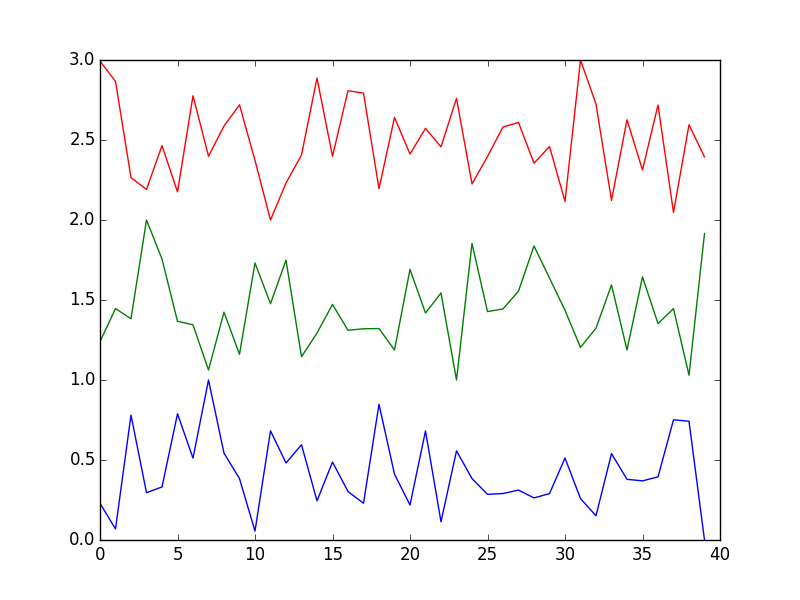
\includegraphics[width=80mm]{icaTest.png}%
            \label{fig:left}%
        }\hfill%
        \subfloat[Signals from the sounds.mat file]{%
        	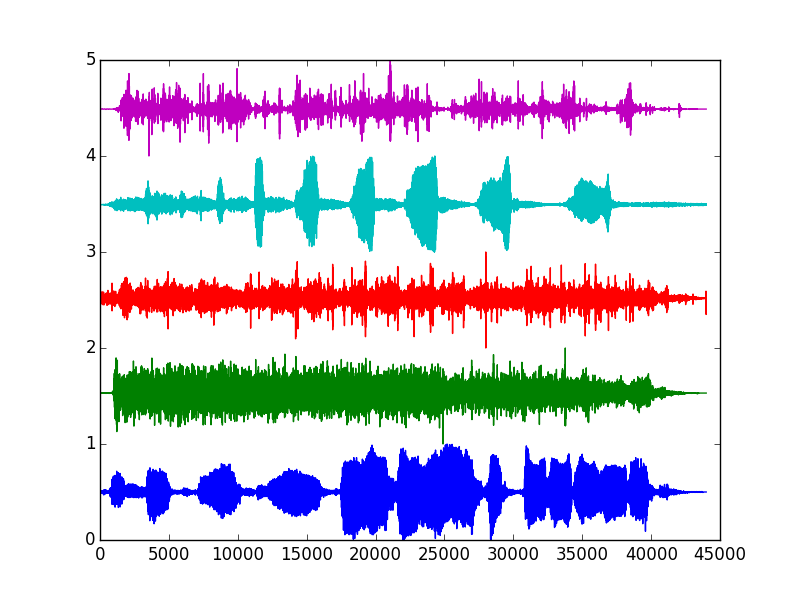
\includegraphics[width=80mm]{sounds.png}%
            \label{fig:right}%
        }
    \caption{\textit{The signals in the two provided input mat files.}}
    \label{fig:default}
\end{figure}

The premise of the experiments in the assignment involved attempting to utilize Independent Component Analysis to take a mixture of signals and separate the mixture into the original signals, with the necessary assumption that the data was non-Gaussian and each component is independent of one other. This implementation of Independent Component Analysis utilized a gradient descent approach to arrive at an unmixing matrix, initially all small random values, that can then be used recover the original signals when applied to the mixture of signals. While the input provided to Independent Component Analysis can be a variety of signals, audio signals are the focus of the experiments described in this paper.

\section{Approach}

My approach to implementing the Independent Component Analysis algorithm leveraged the gradient descent approach exactly as described in the homework prompt. For the sake of concision and brevity, I'm not reproducing it here. My implementation checks for convergence, which is not specified in the assignment prompt, by leveraging the norm of the change to be applied to the unmixing matrix. If the norm is less than a certain convergence constant, \(\epsilon\), I consider the algorithm converged. In the my implementations, I utilize \(\epsilon = 1e^{-10}\).

My only deviation from the mentioned algorithm in the homework prompt was to leverage a learning rate that was determined by a simple, non-adaptive annealing-by-schedule approach rather than a small fixed constant in order to aid convergence. Please refer to Section 3.2.2 for further details.

\section{Experiments}

In order to gauge the correctness of how close the signals were able to be recovered, I utilized the Pearson correlation coefficient. In particular, the Pearson correlation coefficient for a signal compared with itself is 1. Therefore, if a signal is recovered, the correlation will give a decent approximation of how close it is to the original signal. Error below is determined by simply taking 1 minus the Pearson correlation coefficient for a given signal with its corresponding original signal.

Similarly, in order for ensuring stable runs, I selected a fixed, randomly generated mixing matrix A that I knew was not non-invertible or an extremely difficult matrix (e.g. of all zeros) and used it across all experiments.

\subsection{ICA Test File Run}

In order to first perform a sanity check on the algorithm, the implementation was attempted on the provided icaTest.mat file. The run was performed on the parameters described in the assignment prompt (\(\eta=0.01,max\_iterations=1000000\)). Figure 2 describes the results of the run.

\begin{figure}[h]%
	\centering
    	\subfloat[Signals from the icaTest.mat file]{%
        	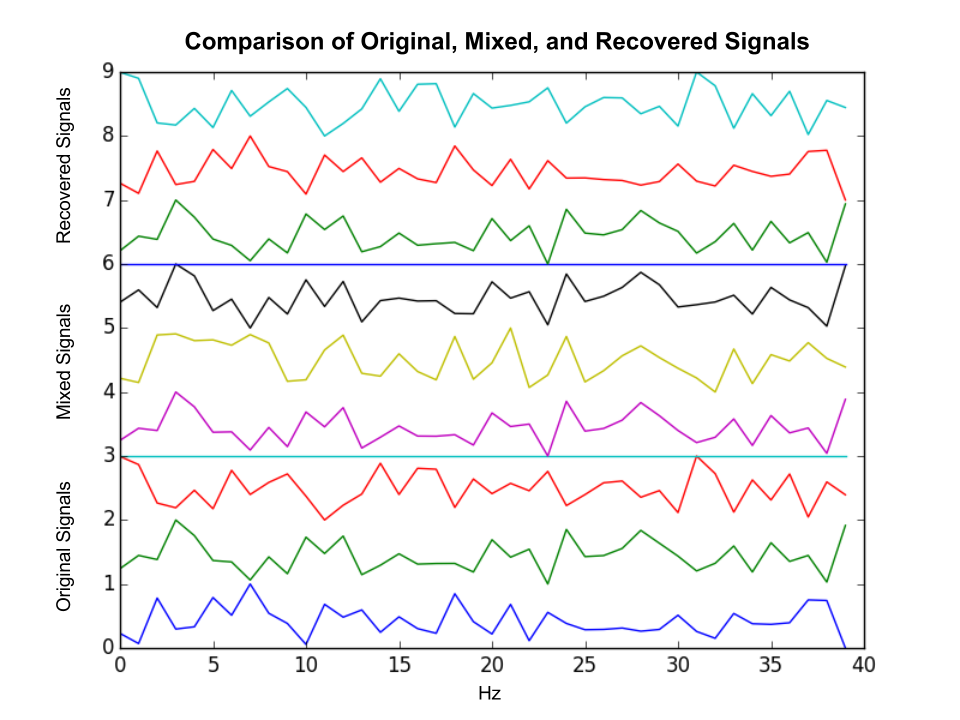
\includegraphics[width=80mm]{icaTestResults.png}%
            \label{fig:left}%
        }\hfill%
        \subfloat[Decrease in error rate over iterations]{%
        	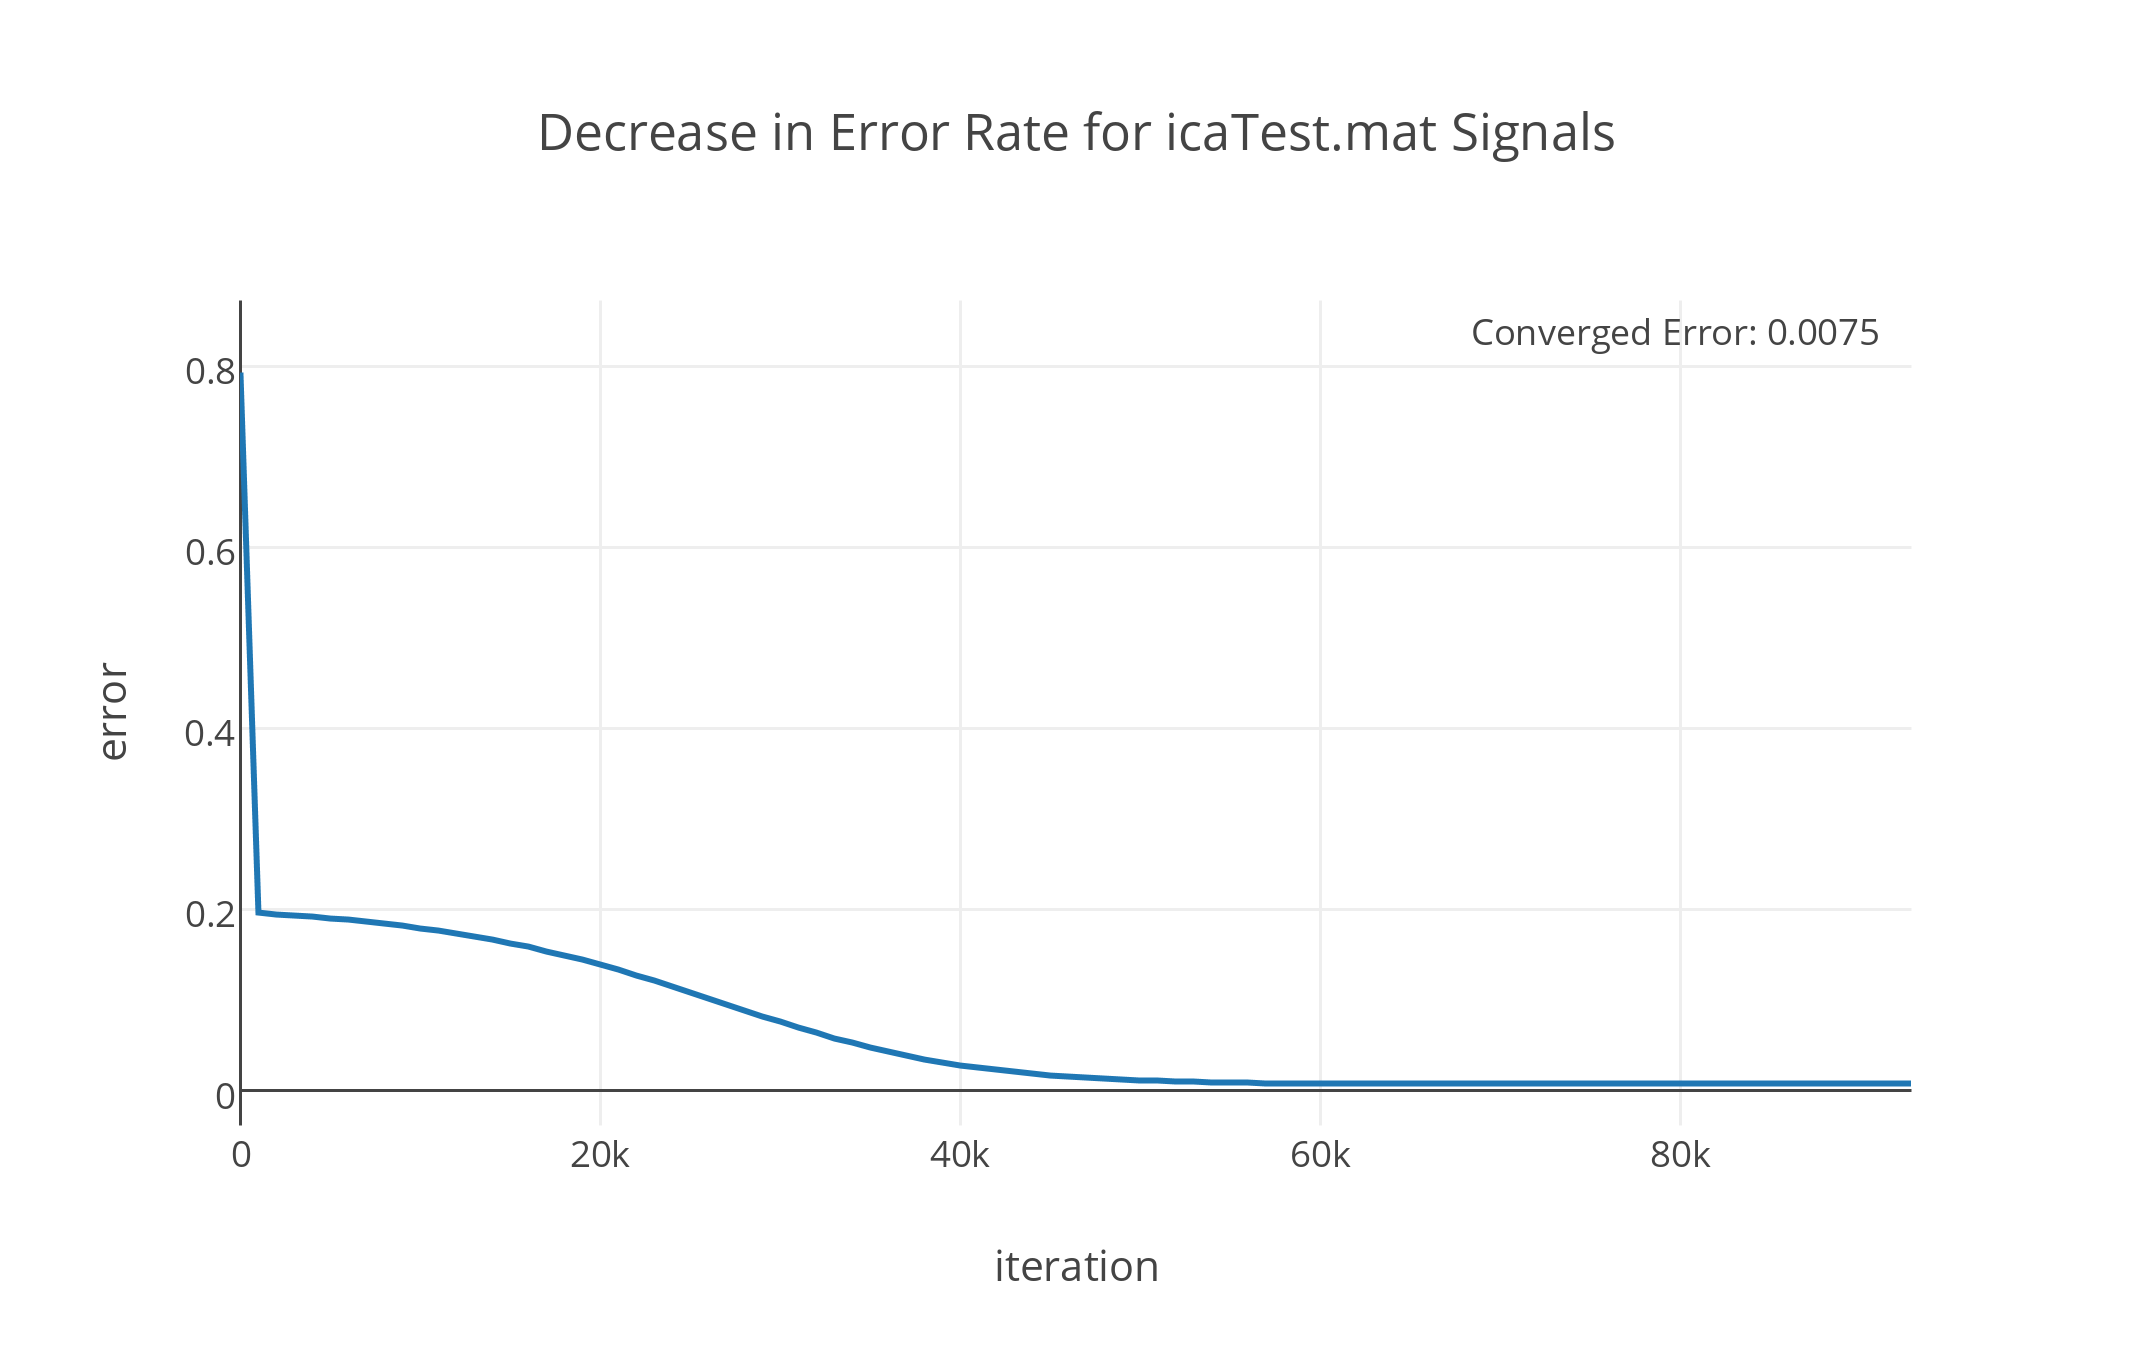
\includegraphics[width=80mm]{decrease_in_error_rate_for_icatestmat_signals__1_.png}%
            \label{fig:right}%
        }
    \caption{\textit{Results of reproducing the original signals after mixing the signals in the icaTest file.}}
    \label{fig:default}
\end{figure}

The signals were able to be recovered with approximately an error rate of less than \(0.01\) within 55000 iterations, achieving a minimum error rate of approximately \(0.0075\). Based on Figure 2b, the error rate decreases gradually after a sharp fall, plateauing at approximately \(0.0075\), though if left alone, it converges at an error of approximately \(0.008420\).

\subsection{Sounds Matrix File Experiments}

Each of the following experiment subsections has three pieces: a description of the setup, a reporting of the results, and an explanation of observation(s) made.

\subsubsection{Constant Learning Rates}

\paragraph{Setup}: After manually running the algorithm on the data several times, I observed the performance of the Independent Component Analysis on three separate runs each at \(\eta \in {0.01, 0.5, 0.95}\) and \(max\_iterations=500000\). The goal of this setup was to observe how the learning rate impacted the convergence of the algorithm, especially given that there are potentially many local minima.

\paragraph{Results} The following three subparagraphs provide detail regarding the results of the experiments based on the setup.
\subparagraph{\textit{Case \(\eta=0.01\)}}- In general, none of the runs converged to an exactly accurate reproduction of signals. Figure 3 provides a plot of the resulting signals as well as their corresponding rate of error reduction.

\begin{figure}%
	\centering
    	\subfloat[Run 1]{%
        	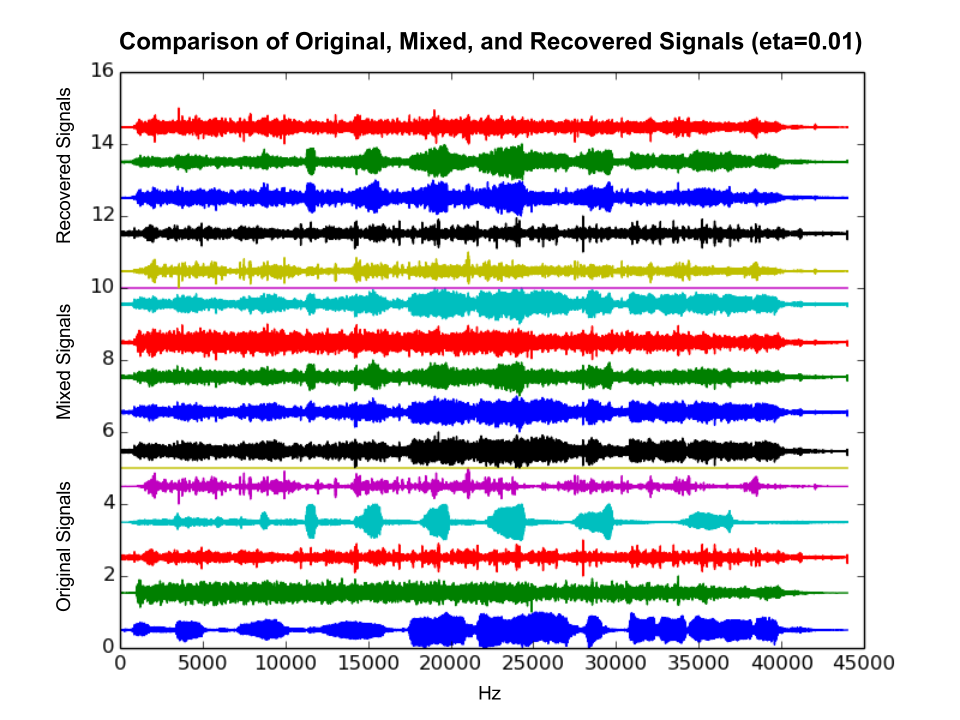
\includegraphics[width=80mm]{eta01-1.png}%
            \label{fig:left}%
        }\hfill%
        \subfloat[Run 2]{%
        	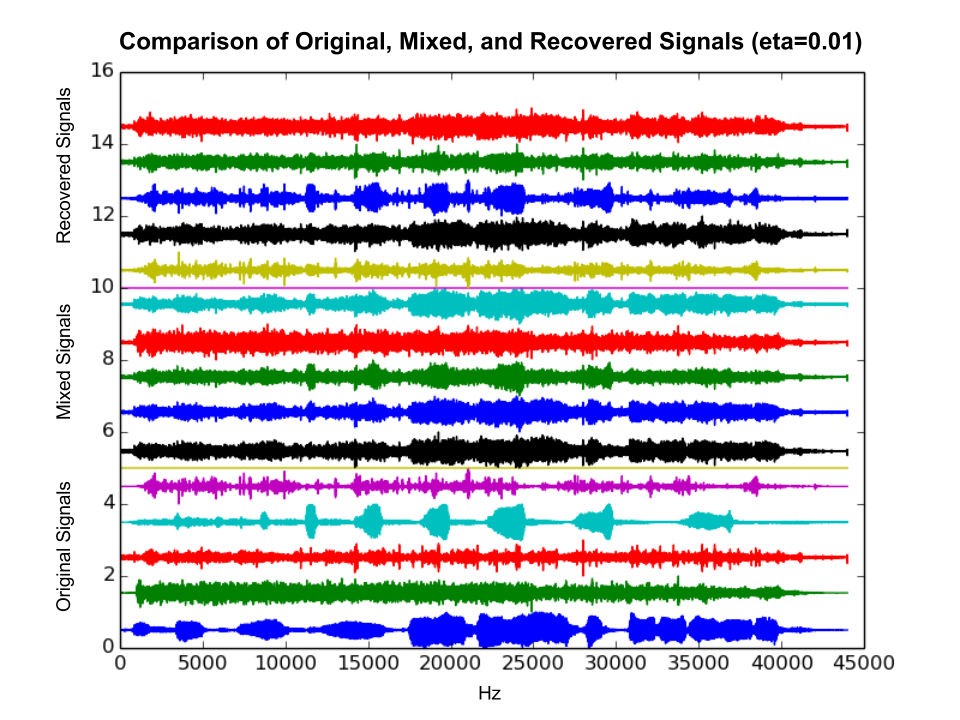
\includegraphics[width=80mm]{eta01-2.png}%
            \label{fig:left}%
        }\hfill%
        \subfloat[Run 3]{%
        	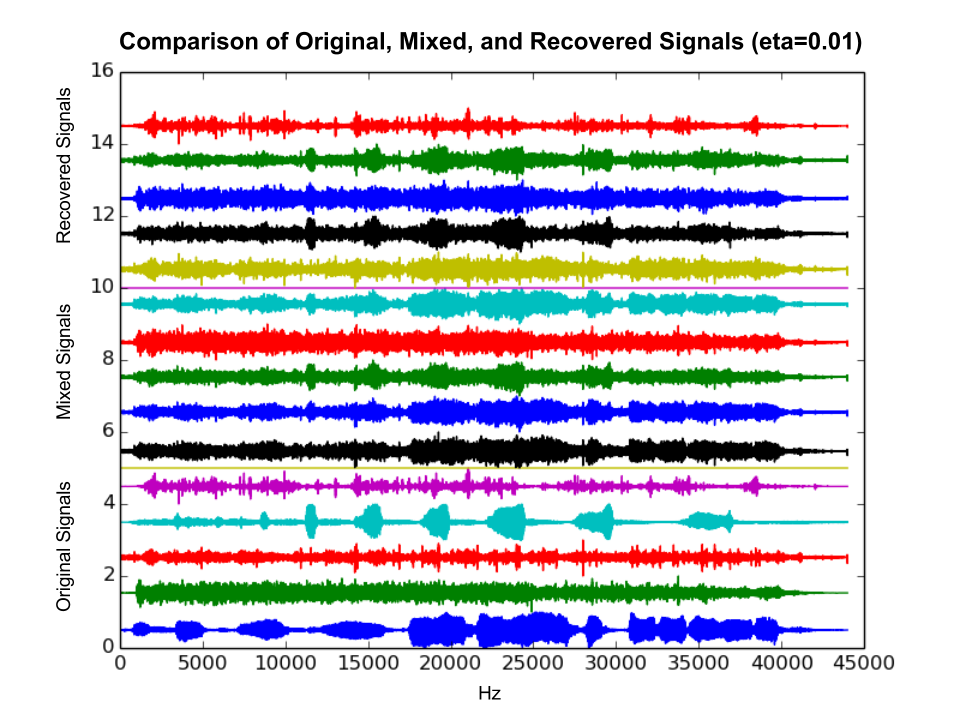
\includegraphics[width=80mm]{eta01-3.png}%
            \label{fig:right}%
        }\hfill%
        \subfloat[Error Rate across Iterations]{%
        	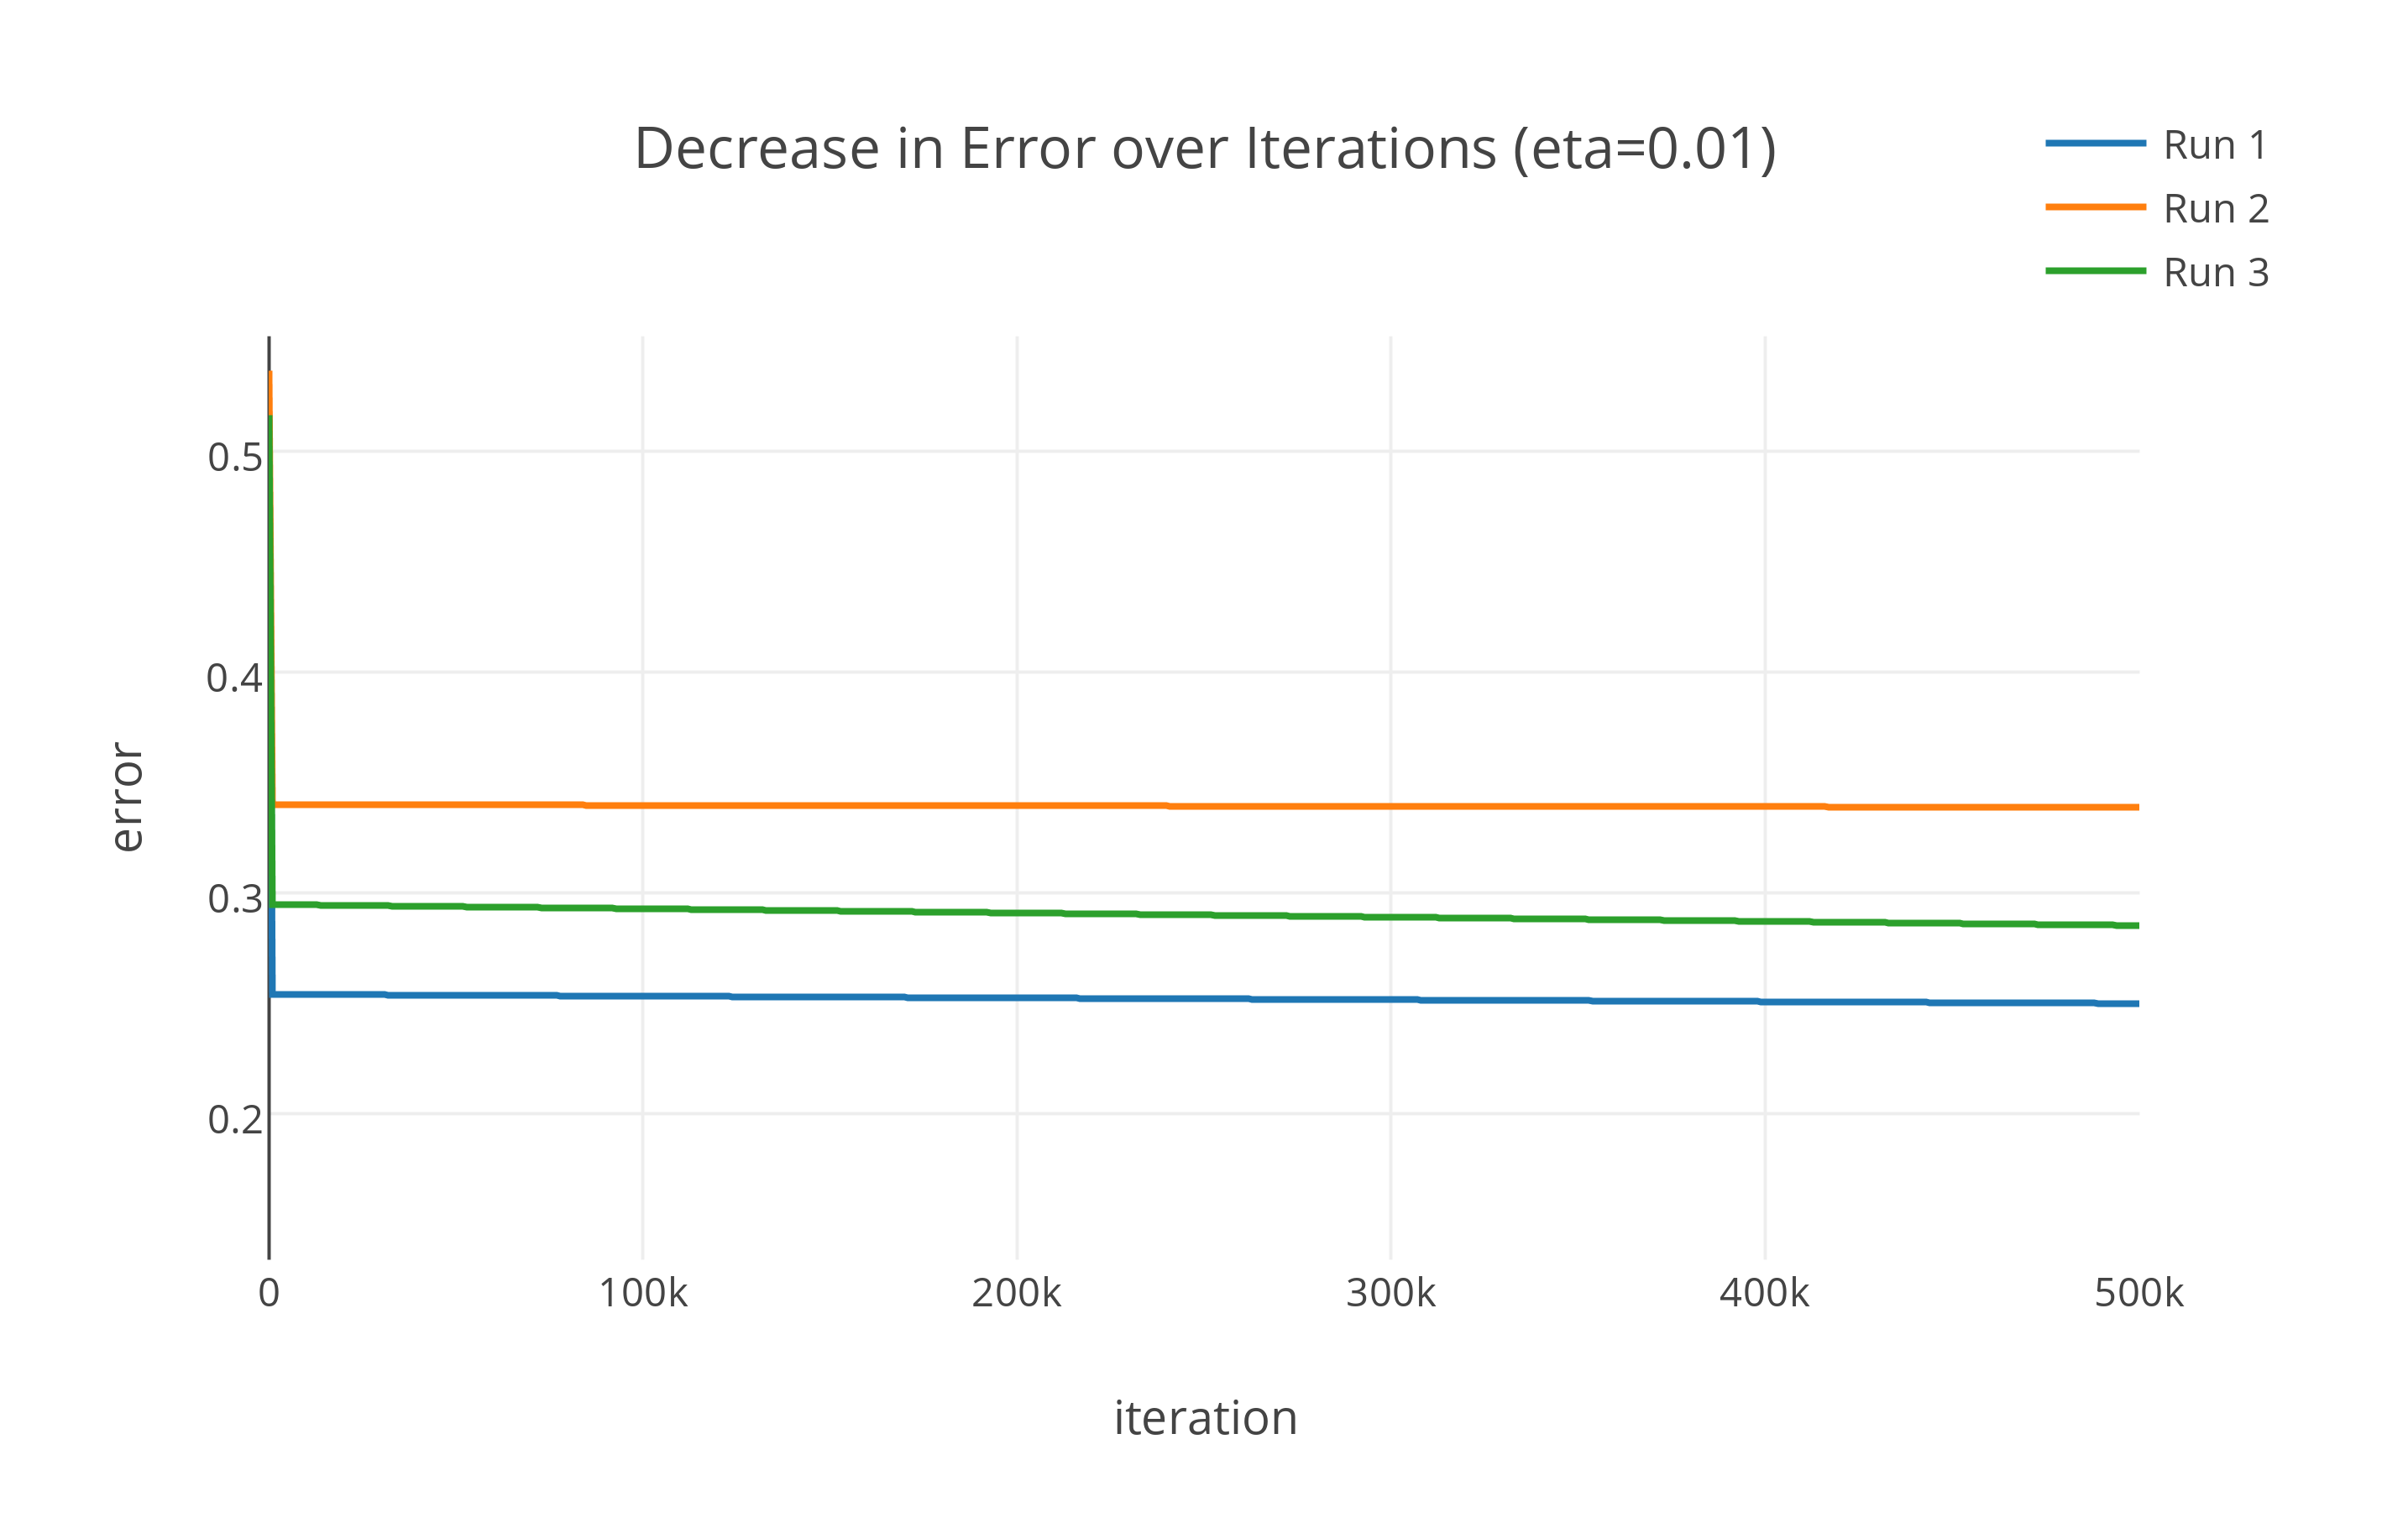
\includegraphics[width=80mm]{eta-01-4.png}%
            \label{fig:right}%
        }
    \caption{\textit{The results of the signal recovery for the three runs with \(\eta=0.01\).}}
    \label{fig:default}
\end{figure} 

In the three runs, the minimum error reached before the maximum number of iterations was \(0.2498\), \(0.3387\), and \(0.28\) respectively. Based on the error rate plot, shown in Figure 3d, the final error rates mentioned above are extremely close to the error rates in the beginning iterations, despite the fact that the algorithm not actually converging. Overall, the rate of approaching a optimal solution is extremely slow and the learning rate seems to be too small for this use case.

\subparagraph{\textit{Case \(\eta=0.5\)}}- The first two of the three runs were able to achieve an average error rage across signals of \(<.01\). Figure 4 provides the results of the signal recovery and their error rates over iteration. 

\begin{figure}%
	\centering
    	\subfloat[Run 1]{%
        	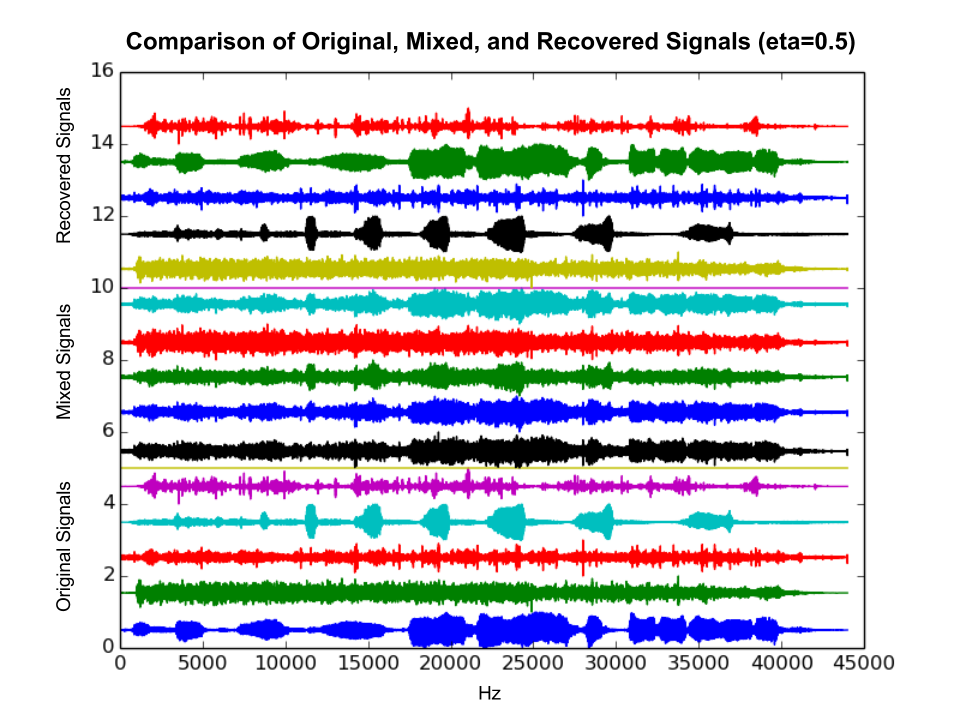
\includegraphics[width=80mm]{eta50-1.png}%
            \label{fig:left}%
        }\hfill%
        \subfloat[Run 2]{%
        	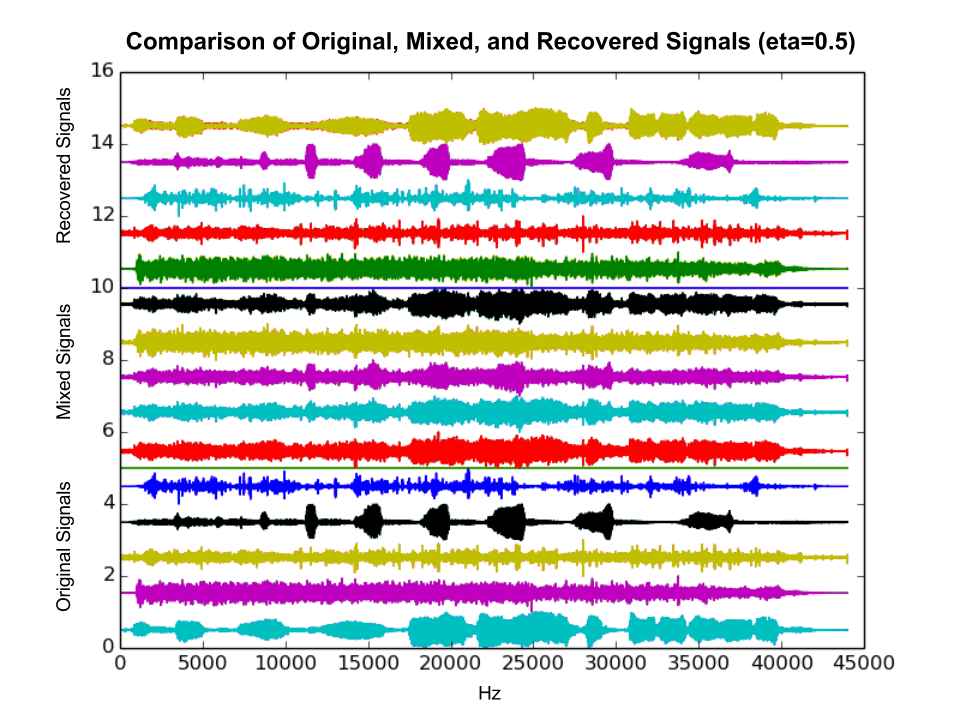
\includegraphics[width=80mm]{eta-50-2.png}%
            \label{fig:left}%
        }\hfill%
        \subfloat[Run 3]{%
        	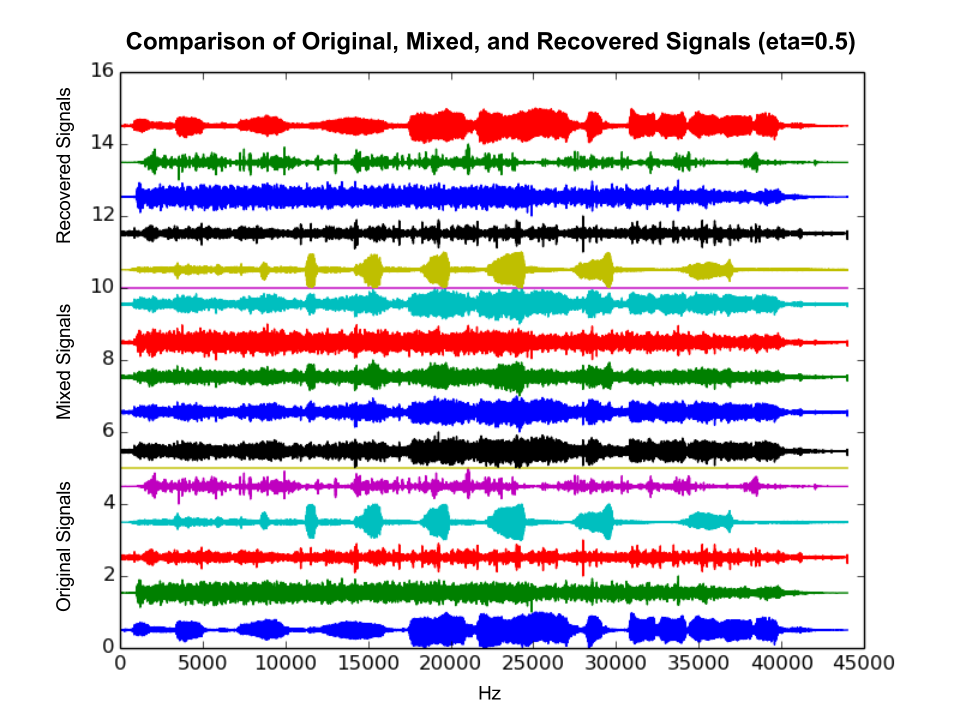
\includegraphics[width=80mm]{eta-50-3.png}%
            \label{fig:right}%
        }\hfill%
        \subfloat[Error Rate across Iterations]{%
        	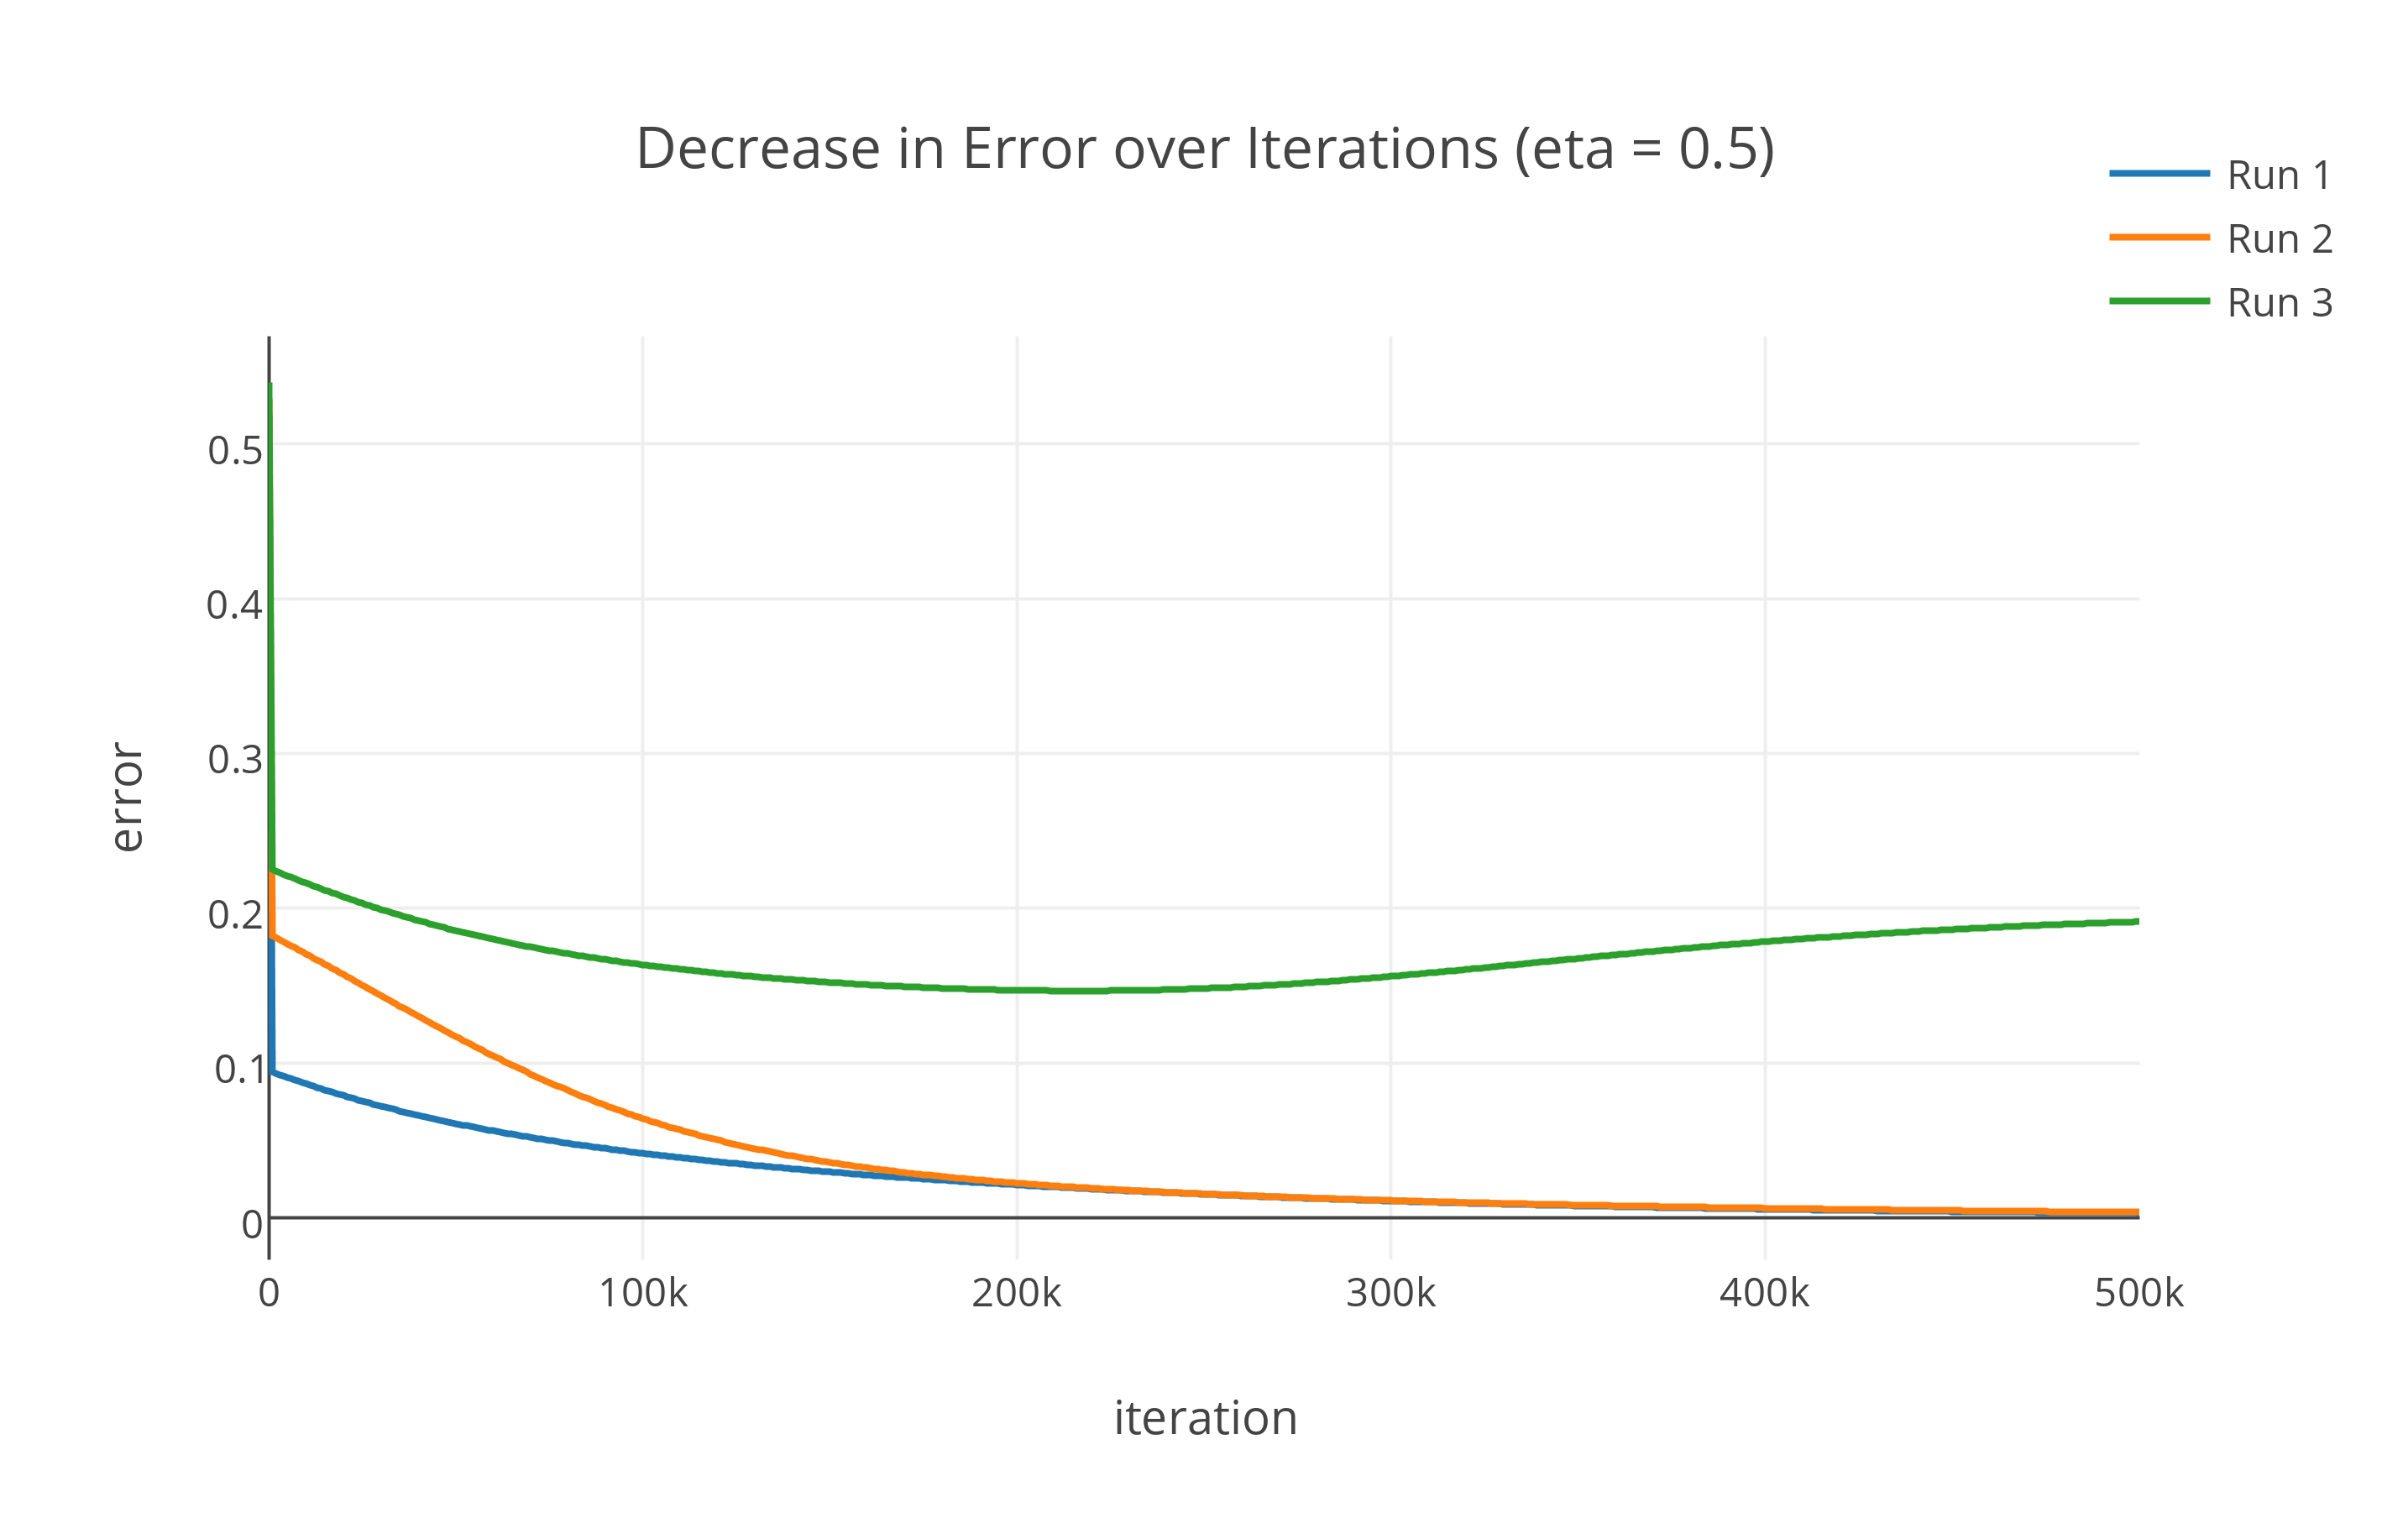
\includegraphics[width=80mm]{eta-50-4.png}%
            \label{fig:right}%
        }
    \caption{\textit{The results of the signal recovery for the three runs with \(\eta=0.50\).}}
    \label{fig:default}
\end{figure} 

The error rates of the first two runs were \(0.003035\) and \(0.003608\) respectively, while the third one had a minimum error rate of \(0.1466\) and finished at an error rate of \(0.1914\). The last run's behavior is either explainable by that it likely reached a local minimum and then began to escape or that it was not able to converge at the minimum and "bounced" out of it. The first two runs, however, seemed to reach an acceptable minimum and were able to reach it at a rate that is much better than the \(\eta=0.01\) cases.

\subparagraph{\textit{Case \(\eta=0.95\)}}- All of my \(\eta=0.95\) cases were able to very closely recover the original signals. Figure 5 provides a depiction of the results of the signal recovery in each of the runs as well as a plot of the error rate over iterations. 

\begin{figure}%
	\centering
    	\subfloat[Run 1]{%
        	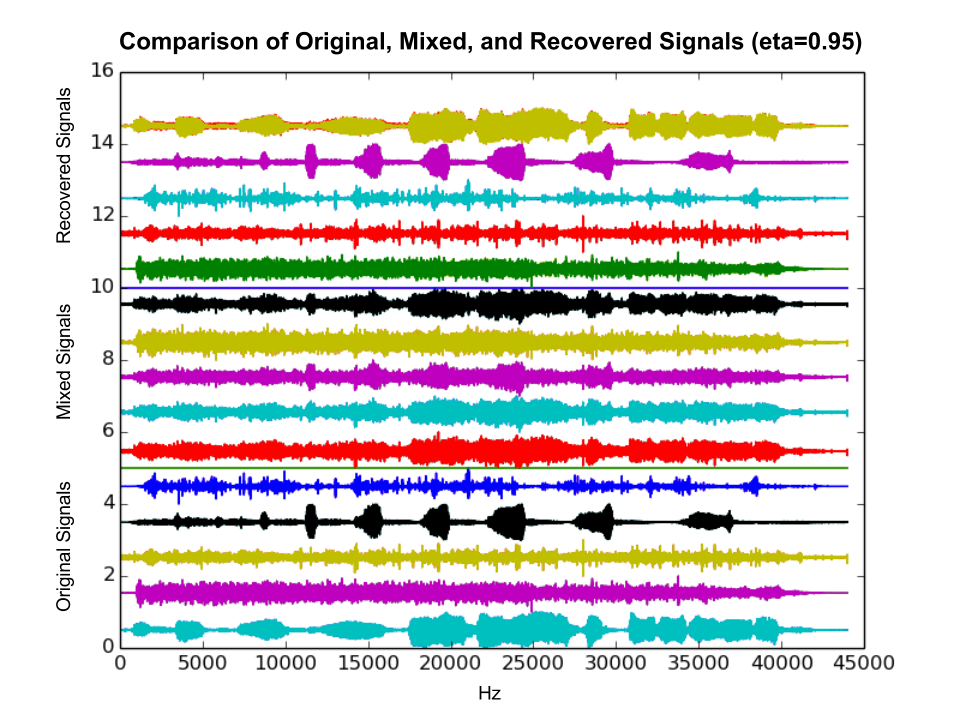
\includegraphics[width=80mm]{eta-95-1.png}%
            \label{fig:left}%
        }\hfill%
        \subfloat[Run 2]{%
        	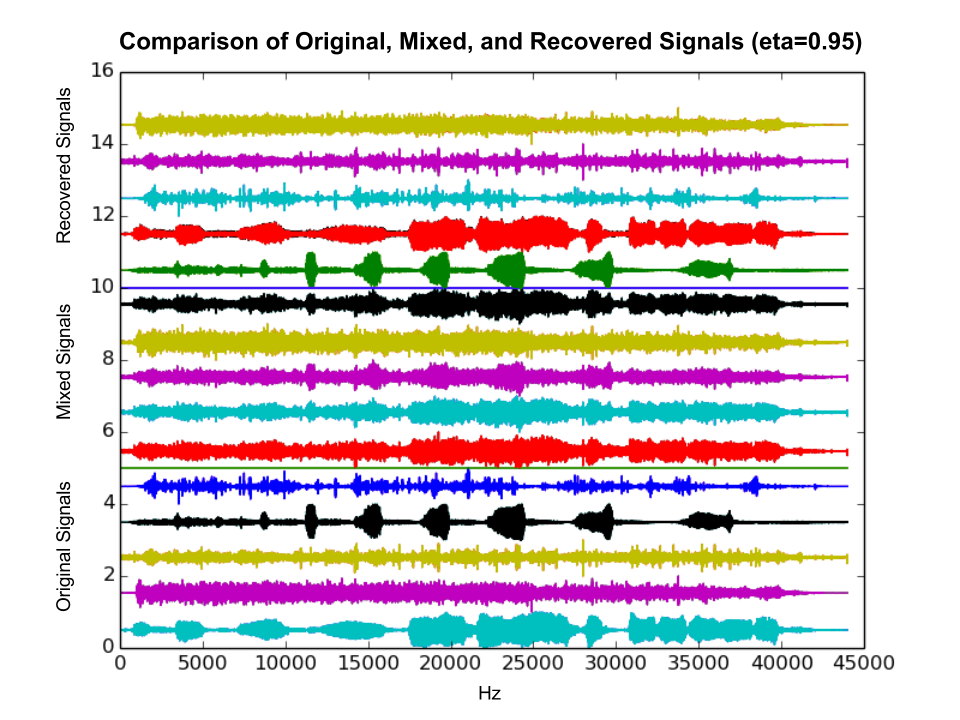
\includegraphics[width=80mm]{eta-95-2.png}%
            \label{fig:left}%
        }\hfill%
        \subfloat[Run 3]{%
        	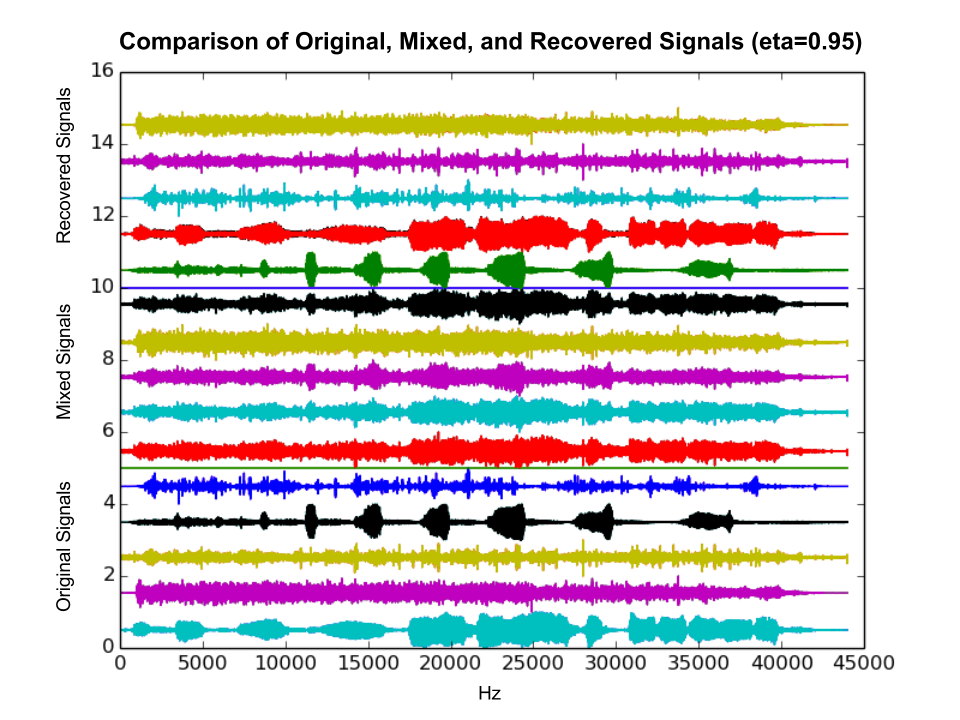
\includegraphics[width=80mm]{eta-95-3.png}%
            \label{fig:right}%
        }\hfill%
        \subfloat[Error Rate across Iterations]{%
        	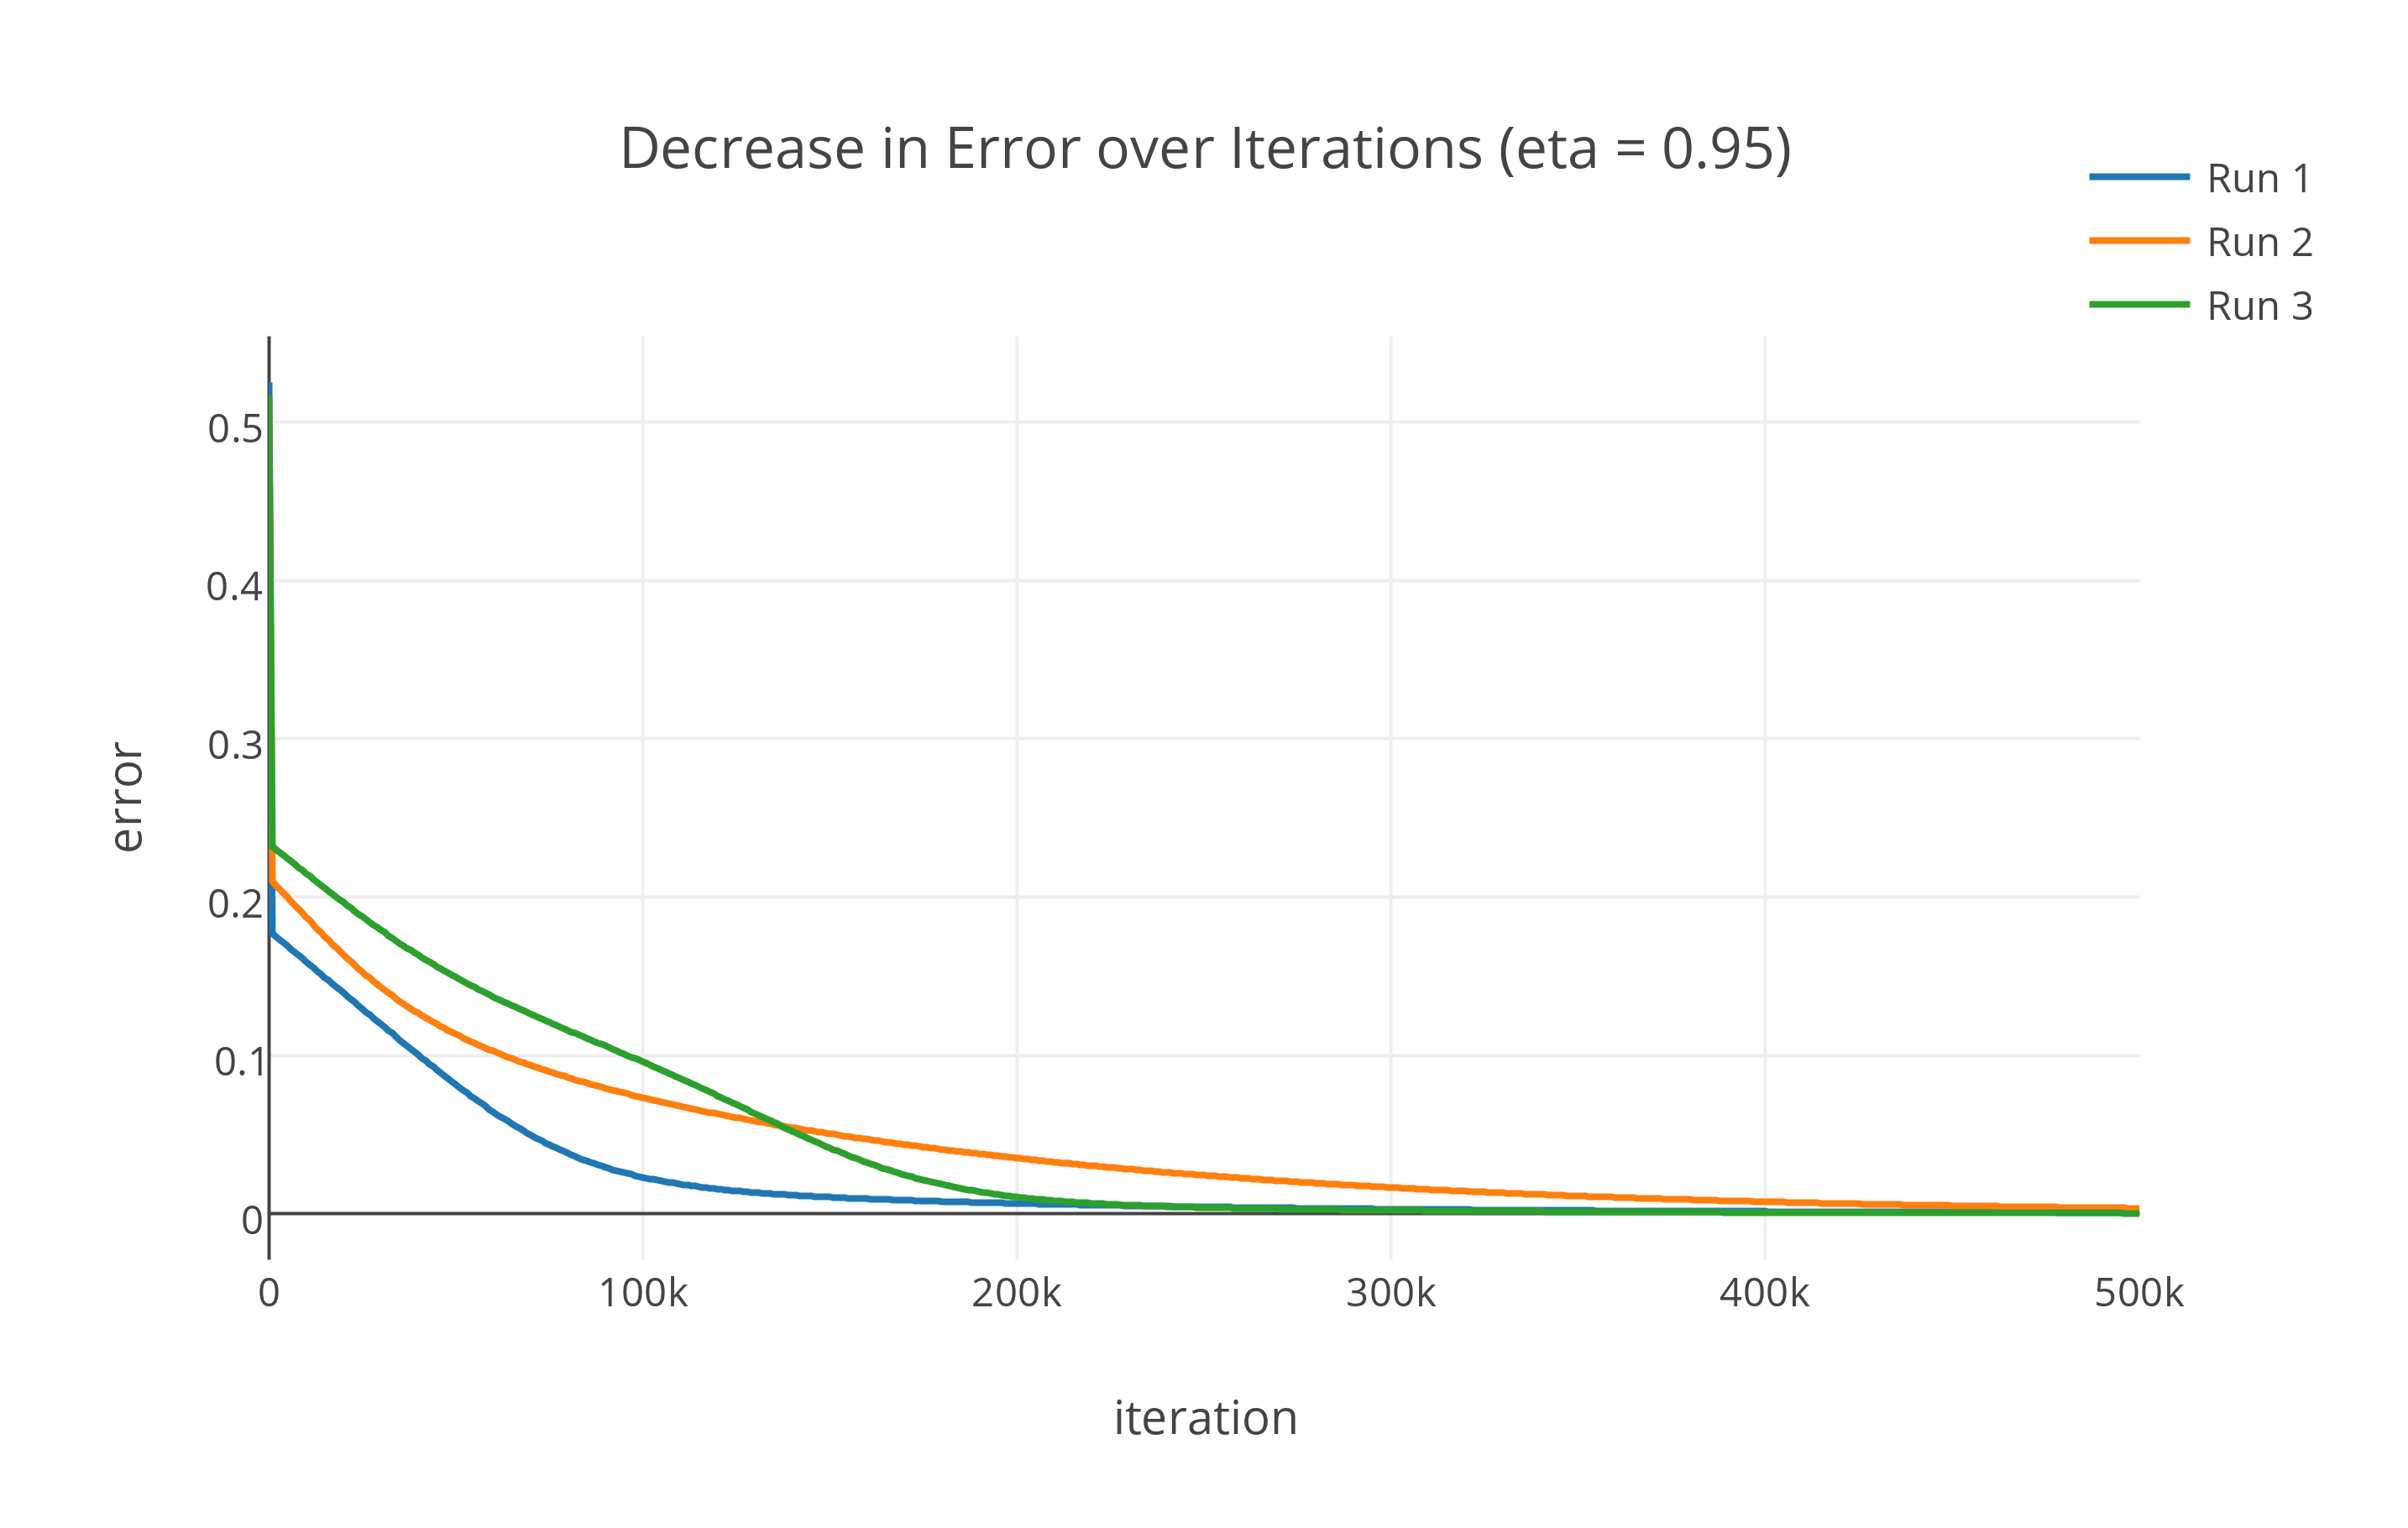
\includegraphics[width=80mm]{eta-95-4.png}%
            \label{fig:right}%
        }
    \caption{\textit{The results of the signal recovery for the three runs with \(\eta=0.95\).}}
    \label{fig:default}
\end{figure} 

All three runs reached an error rate \(<0.01\). The final error rates of each of the three runs were \(0.0008307\), \(0.003504\), and \(0.0003938\). The \(\eta=0.95\) runs performed significantly better than the other runs in terms of both speed to reach an error rate less than \(0.01\). Based on the curvature in Figure 5, the \(\eta=0.95\) runs expectedly had their error rate decrease at a steeper rate than the other runs as well. 

\paragraph{Observations}

As expected, none of the runs were duplicates of one another. Each run is different in how quickly convergence is accomplished or an extremely small error rate (e.g. \(< 0.01\) is reached). This is largely due to the fact that the algorithm begins randomly selecting an unmixing matrix, where the unmixing matrix could be selected at a location which is close to a less ideal local minima. This initial randomized selection of the start unmixing matrix impacts the overall number of iterations that need to be taken for a good solution and, based on the parameters, the quality of the solution as well.

Another major observations is the difference in complexity between the signals in the icaTest.mat file and the sounds.mat file. Given the complexity and the length, the Independent Component Analysis algorithm is more likely to get potentially stuck at local minima with the signals in sounds.mat. Therefore, the small 0.01 learning rate that was satisfactory for approximate recovery of the signals in the simpler case might not at all be sufficient for more complex signals and situations, in general. 

The complexity makes the choice of learning rate a non-trivial problem. If proceeding with slow learning rates, if stuck at a local minima, it can be difficult to get out of the local minima. In addition, the convergence with small learning rates could just be extremely slow. This is likely what occurred with some of the runs in the \(\eta=0.01\) case. On the other hand, faster learning rates, while providing the ability to potentially avoid local minima or quickly proceed, can lead an algorithm to bounce around minima and not actually converge at a minimum. This is likely what happened with the cases in \(\eta=0.5\) and \(\eta=0.95\) that did not exactly converge to or, at least, reach an error of less than \(1\%\). As a result, in practice, a high constant rate, such as 0.95, might not be suitable.

More sophisticated techniques for learning rates are ideal. In particular, annealing techniques that can start with larger learning rates and then "cool" to smaller ones could potentially help. In particular, the larger rates could be useful in searching appropriate optima while the smaller rates, when cooled, can be useful for converging to an appropriate optimum. Other techniques such as momentum, which leverages the search's inertia to help reduce the oscillations in the search, can be similarly useful.

\subsubsection{Dynamic Learning Rates}

\paragraph{Setup}

In order to attempt a more dynamic learning rate but limit the number of new parameters introduced, I leveraged a simple, non-adaptive version of annealing. My implementation's source is from a Williamette University course\footnote{http://www.willamette.edu/\~gorr/classes/cs449/momrate.html}. The annealing approach, a simplification of the one mentioned in the "Learning Rate Schedules For Faster Stochastic
Gradient Search"\footnote{http://citeseerx.ist.psu.edu/viewdoc/download?doi=10.1.1.42.2884\&rep=rep1\&type=pdf} paper, computes the learning rate, \(\eta\), at each iteration \(i\) based on the following method:

\begin{align*} 
\begin{split}
\eta(i) = \eta_0 (\frac{T}{T+i})
\end{split}					
\end{align*}

I leveraged a \(max\_iterations\) value of 500000, started with \(\eta_0=.99\) since the literature recommends a high value for \(\eta_0\) in the context of annealing, and kept the T parameter at 200000 given the context of the experiments. With these configurations, I executed three runs.

\paragraph{Results}

All of the signals were able to be recovered with a high degree of accuracy. Figure 6 shows the results of the experiment.

\begin{figure}%
	\centering
    	\subfloat[Run 1]{%
        	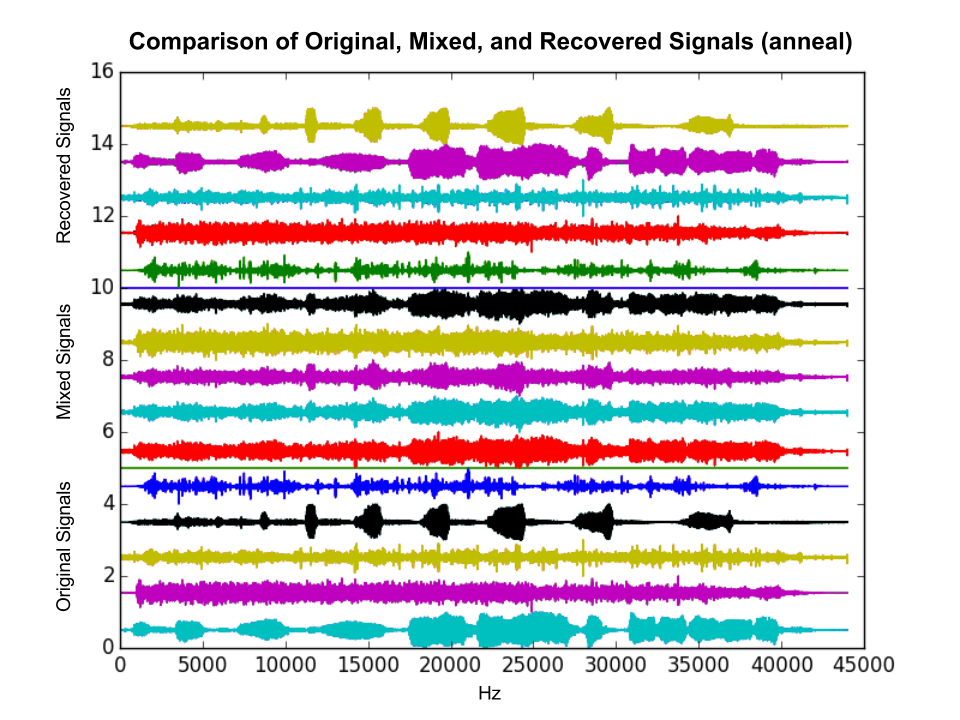
\includegraphics[width=80mm]{anneal-1.png}%
            \label{fig:left}%
        }\hfill%
        \subfloat[Run 2]{%
        	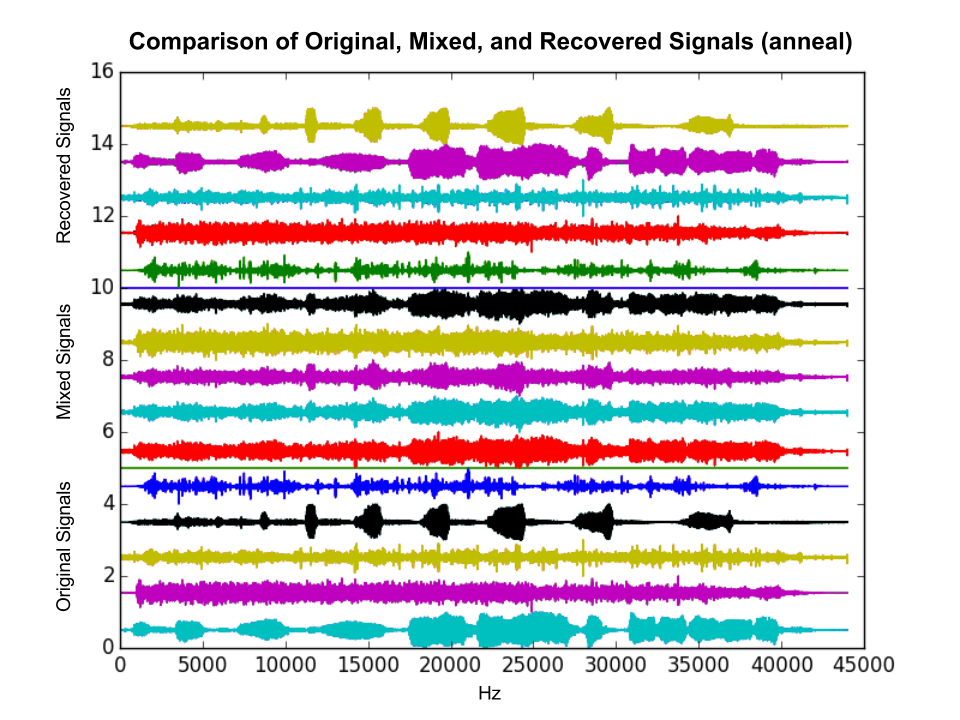
\includegraphics[width=80mm]{anneal-2.png}%
            \label{fig:left}%
        }\hfill%
        \subfloat[Run 3]{%
        	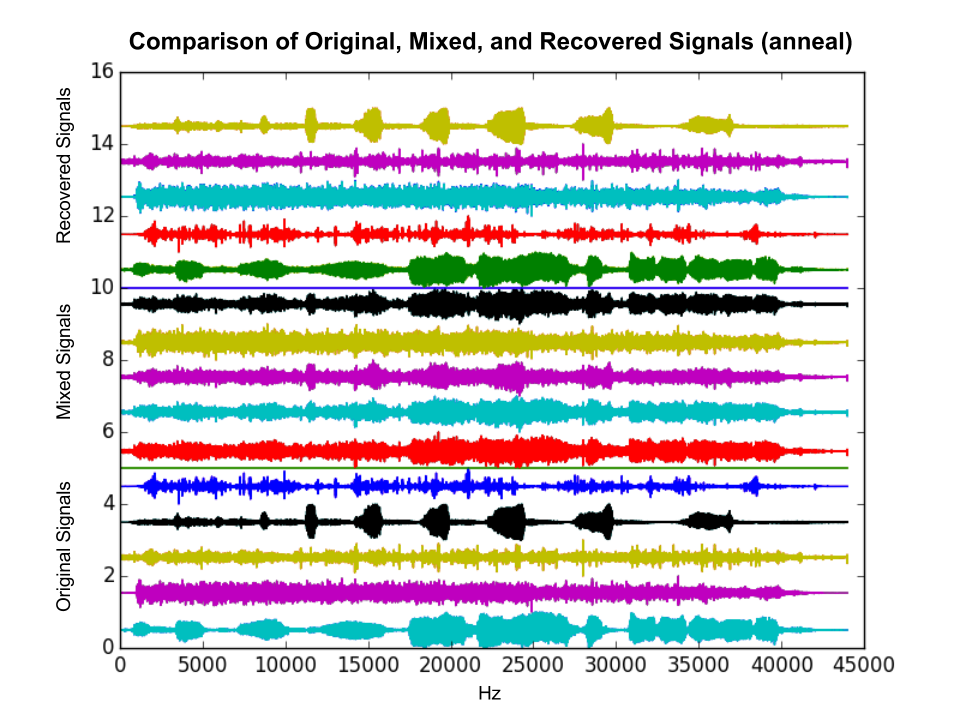
\includegraphics[width=80mm]{anneal-3.png}%
            \label{fig:right}%
        }\hfill%
        \subfloat[Error Rate across Iterations]{%
        	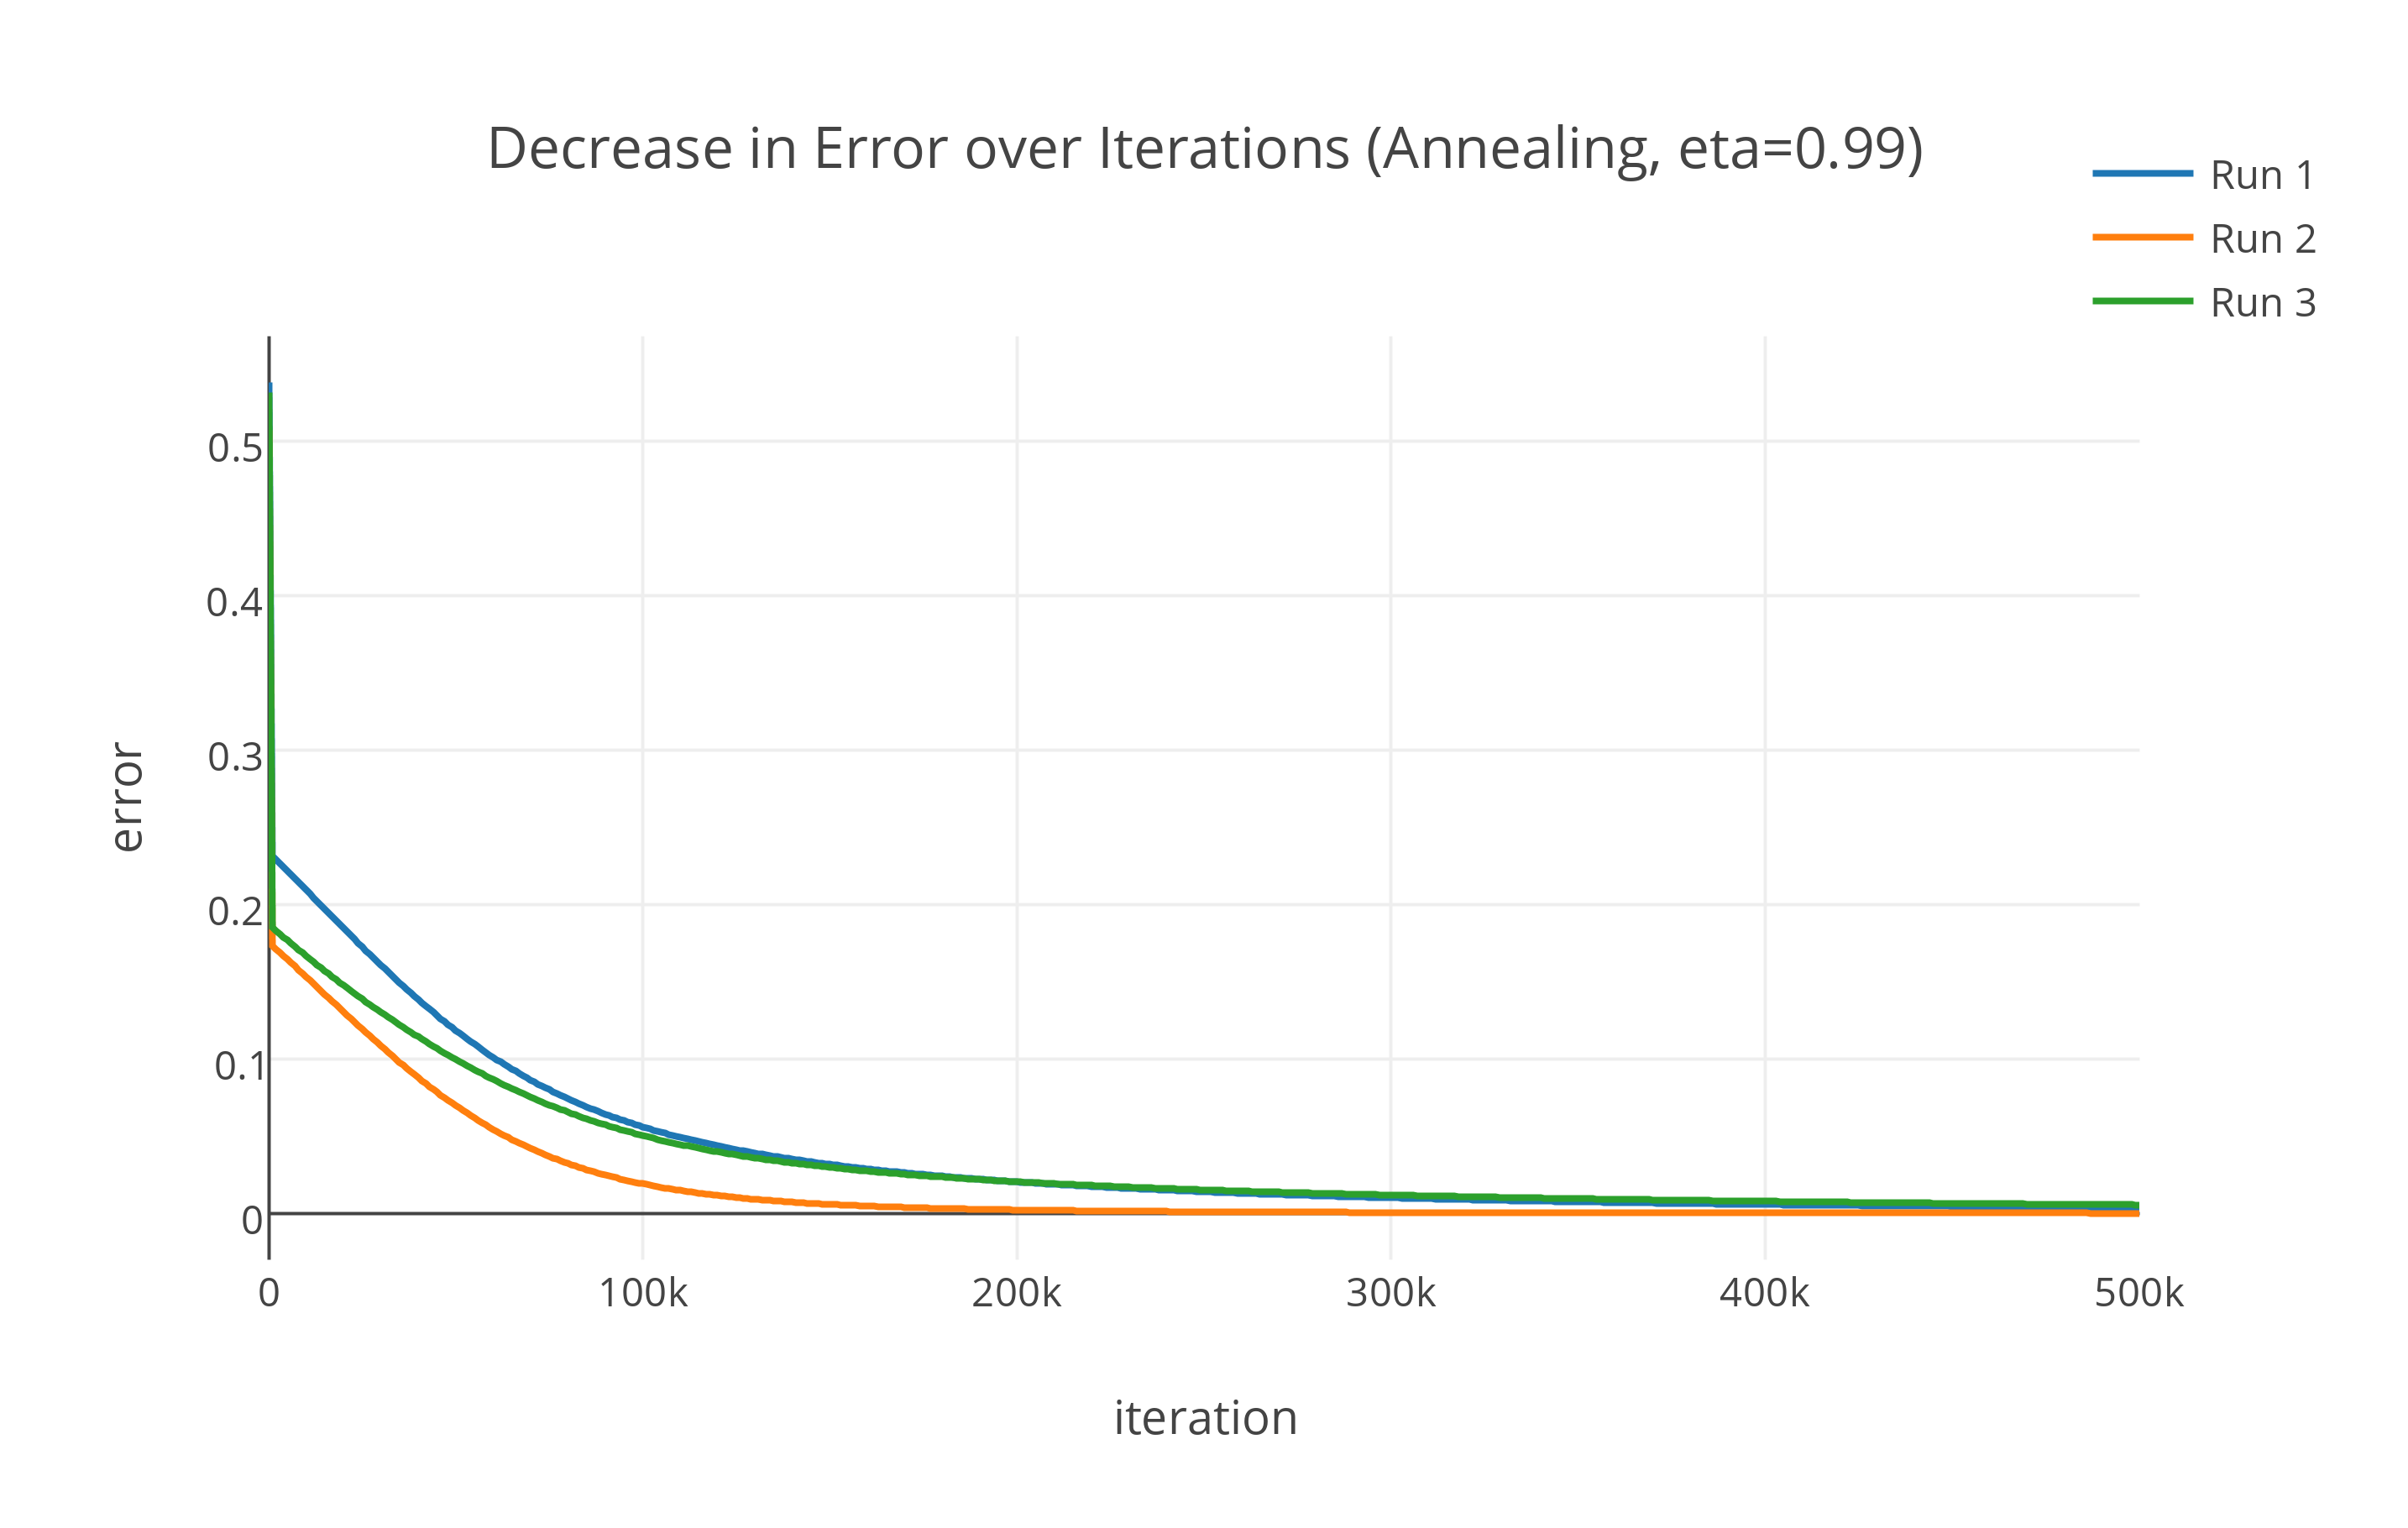
\includegraphics[width=80mm]{anneal-4.png}%
            \label{fig:right}%
        }
    \caption{\textit{The results of the signal recovery for the three runs with the simple annealing at \(\eta_0=0.99\).}}
    \label{fig:default}
\end{figure}

Each run had an error rate less than \(0.01\). The error rates for the three runs were \(0.003791\), \(0.0003444\), and \(0.005757\) respectively. The curvature of the error rate lines for each of the runs in Figure 6d followed the same kind of pattern : an initial relatively steep rate of drop that slows down as the number of iterations increase (i.e. due to the decreasing learning rate). Of all of the runs, in terms of final error rate, the anneal runs performed better than the \(\eta=0.01\) and \(\eta=0.5\) cases but slightly worse than the \(\eta=0.95\) runs. 

\paragraph{Observations}

The steep and slow patterns likely show both an exploratory phase and a convergence phase. The main point of the anneal case is to use a high learning rate that would first explore different optimum and the converge to a good optimum as the learning rate slows. Though the \(\eta=0.95\) may have achieved final results that were better than that of the anneal case, annealing will be a better alternative in the general case. In particular, a high learning rate may be less than ideal for the reasoning mentioned in the Observations segment in Section 3.2.1. The data set provided here may simply have less poor local optima or I may not have encountered them in the number of times that I've run the experiments.

In addition, the simple annealing approach, based on the Williamette University notes, could probably be improved itself. In particular, the \(T\) constant used creates another parameter for the user to tweak. The algorithm could use approaches that are more adaptive to reduce the impact of user defined parameters (e.g. the \(T\) in this case) on the performance. 

\subsubsection{Signal Variation}

Tuned appropriately, all provided signals were able to be retrieved quite well. The assignment implies that some signals might be more difficult to recover than the others. However, based on the results from the above two sections, I was unable to observe that any particular signal was particularly difficult to retrieve or that any particular signal was difficult to separate from the mixed signals. While I agree that the complete recovery of each signal may not happen equivalently, based on the experiments above alone, I saw enough variation while observing each component during each run for me to conclude that I was unable to make any conclusion regarding a signal being more difficult than the other.

However, intuitively, I expected that if two signals are more similar to one another, separating them might be easier than two signals are that different from one another. The source of my intuition is the extremity of the above statement - trying to separate a mixture of two signals that are identical. I would expect that situation to be easier.

\paragraph{Setup}

I selected signal 0 and 1 as two signals that seemed different from one another. I selected signal 2 and 4 as two signals that seemed similar to me. I mixed the two using the same matrix and ran the separation process three times each. I ignored all results where I happened to get lucky to fall right next (i.e. extremely close enough that in a few iterations the error rate would be less than 0.01) to the solution by the random initialization of W.

\paragraph{Results}

As before, I was able to separate all of the signals with a little error (i.e. \(<0.01\)). Table 1 describes the results of the experiments and Figure 7 shows the separated signals. Note that the iterations are in recorded in granularity of 1000s due to performance constraints.

\begin{table}[H]
\centering
\begin{tabular}{|c|c|c|}
\hline
\textbf{Case} & \textbf{Run} & \textbf{Iterations to \(< 0.01\)} \\\hline
 & 1 & 38000 \\\cline{2-3} 
2,4 Signals & 2 & 24000 \\\cline{2-3}
 & 3 & 46000 \\\hline
 & 1 & 157000 \\\cline{2-3}
0,1 Signals & 2 & 161000 \\\cline{2-3}
 & 3 & 446000 \\\hline
\end{tabular}

\caption{\label{tab:widgets} Results for the 2,4 signal separation and 0,1 signal separation listing the iterations to reach error less than 0.01.}
\end{table}

\begin{figure}%
	\centering
    	\subfloat[2,4 Signals Run 1]{%
        	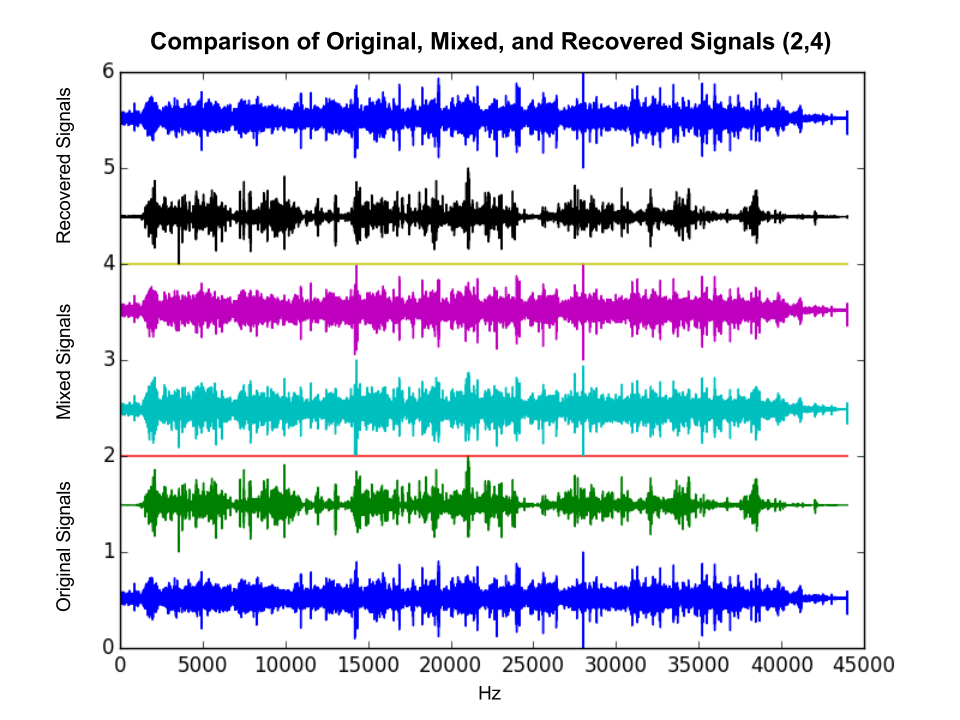
\includegraphics[width=55mm]{exp3-2-4-1.png}%
            \label{fig:left}%
        }\hfill%
        \subfloat[2,4 Signals Run 2]{%
        	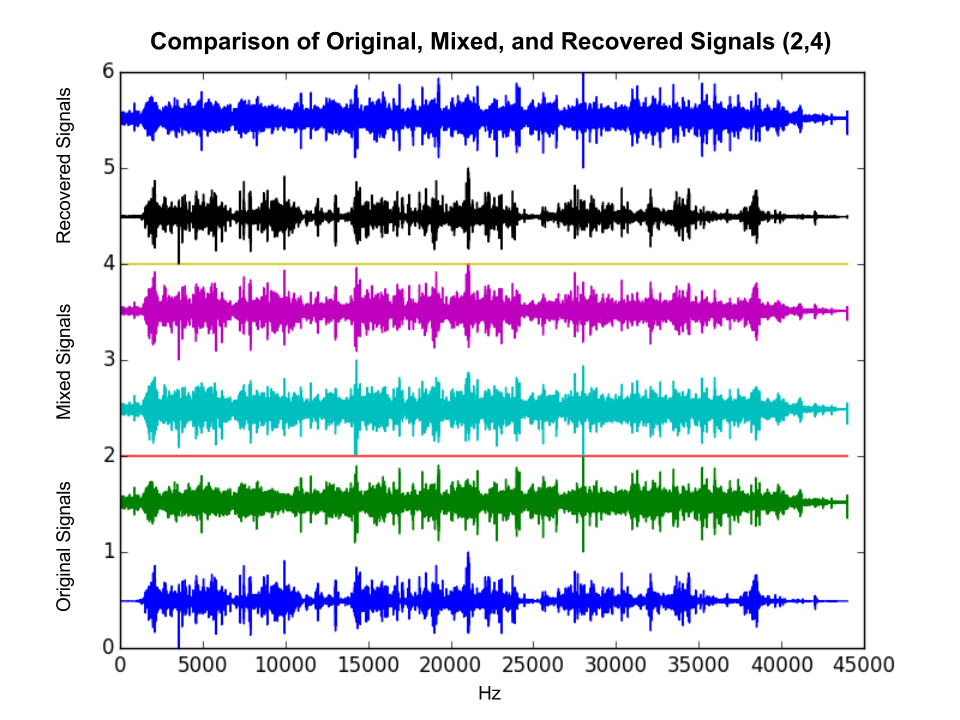
\includegraphics[width=55mm]{exp3-2-4-2.png}%
            \label{fig:left}%
        }\hfill%
        \subfloat[2,4 Signals Run 3]{%
        	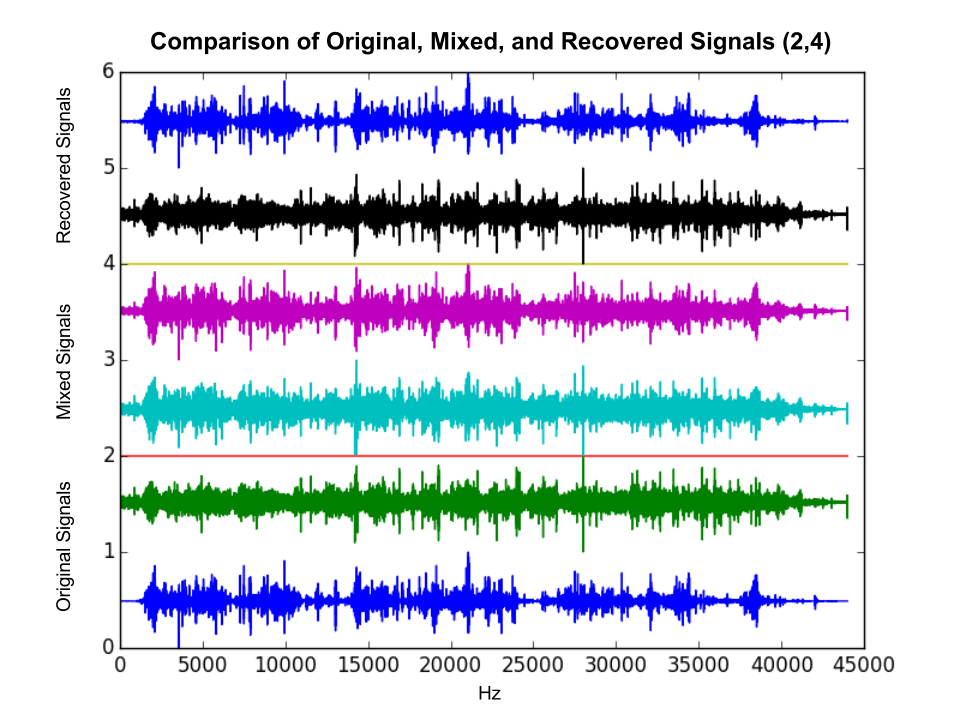
\includegraphics[width=55mm]{exp3-2-4-3.png}%
            \label{fig:right}%
        }\hfill%
    	\subfloat[0,1 Signals Run 1]{%
        	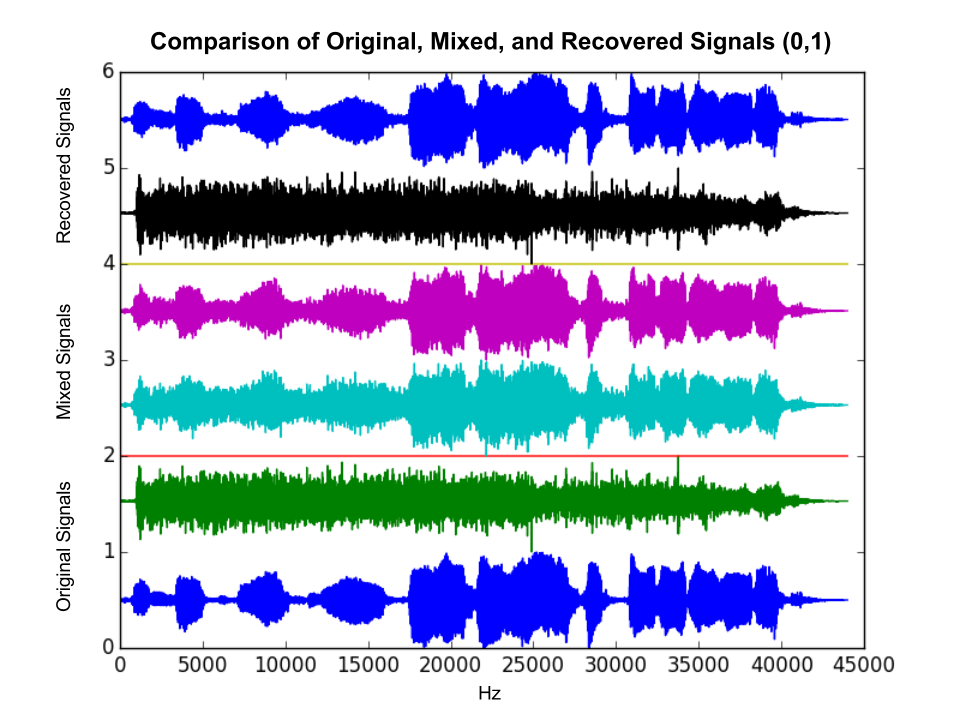
\includegraphics[width=55mm]{exp3-0-1-1.png}%
            \label{fig:left}%
        }\hfill%
        \subfloat[0,1 Signals Run 2]{%
        	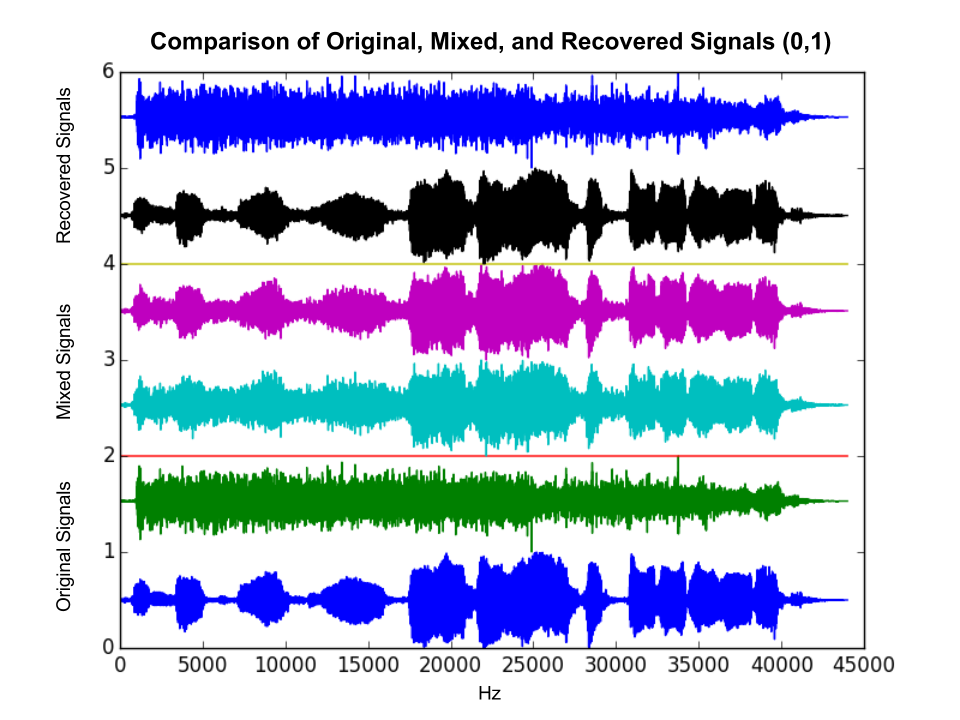
\includegraphics[width=55mm]{exp3-0-1-2.png}%
            \label{fig:left}%
        }\hfill%
        \subfloat[0,1 Signals Run 3]{%
        	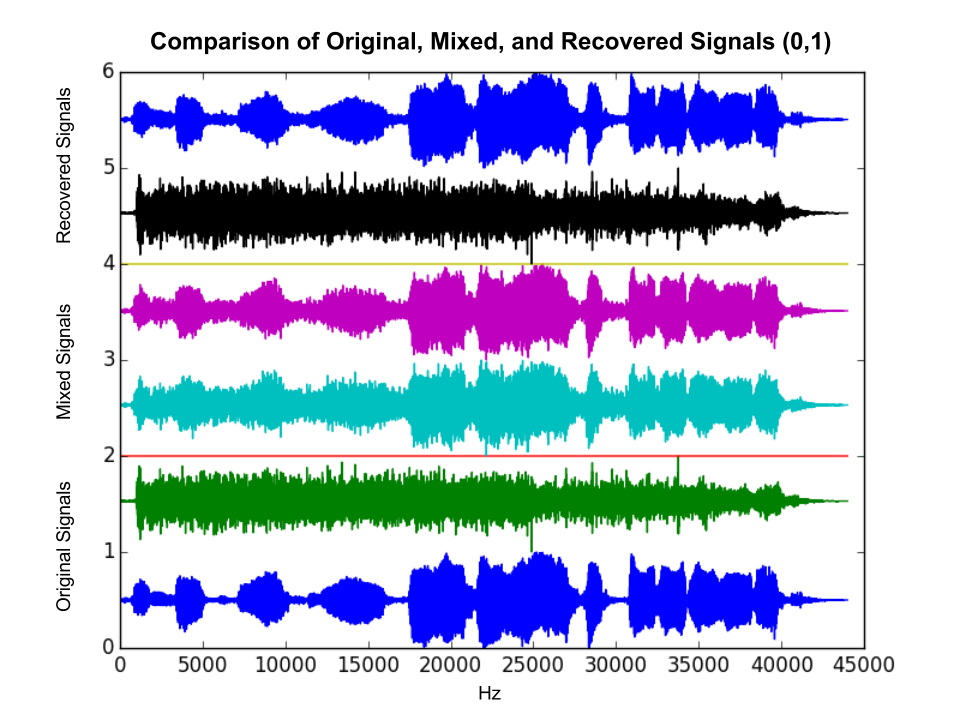
\includegraphics[width=55mm]{exp3-0-1-3.png}%
            \label{fig:right}%
        }
    \caption{\textit{Separation results for the 2,4 signals mixture and 0,1 signals mixture}}
    \label{fig:default}
\end{figure}

As Table 1 shows, the number of iterations that was taken to reach an error rate less than 0.01 is significantly less for 2,4 signals than the 0,1 signals.

\paragraph{Observations}

Based on the small sample above, I was able to observe that the results aligned with the expectations that I mentioned in the Setup segment. I believe that the similarity between the two signals in the 2,4 case lends to an easier separation than in the 0,1 signals case. However, I'm not sure that it is enough to conclude that this is exactly the case. Given the randomized start and the number of samples, the results found in this experiment could have been impacted by other variables. My reasoning and this small result sample provides an avenue for further investigation. To further confirm the results found here, the actual experiment needs to be run more times to confirm the phenomenon from a large result set. 

\section{Concluding Notes}

I'm interested in the degree at which Independent Component Analysis scales. For the five signal cases, each representing four-second samples of audio, in the experiments above, the actual signal separation process took significant time. Though it might be the implementation or the algorithm that might be lacking, I wonder how a similar approach to Independent Component Analysis might perform in the context of more, longer audio signals (e.g. even a small one such as 10 signals of 20 seconds each). Intuitively, it seems there is a lot of work in considering every single point in each of the signals. For future work, I would be interested in tackling or investigating how Independent Component Analysis or simply the process of separating components can scale or be optimized.

\end{document}
